% Options for packages loaded elsewhere
\PassOptionsToPackage{unicode}{hyperref}
\PassOptionsToPackage{hyphens}{url}
%
\documentclass[
  ,man]{apa6}
\usepackage{amsmath,amssymb}
\usepackage{iftex}
\ifPDFTeX
  \usepackage[T1]{fontenc}
  \usepackage[utf8]{inputenc}
  \usepackage{textcomp} % provide euro and other symbols
\else % if luatex or xetex
  \usepackage{unicode-math} % this also loads fontspec
  \defaultfontfeatures{Scale=MatchLowercase}
  \defaultfontfeatures[\rmfamily]{Ligatures=TeX,Scale=1}
\fi
\usepackage{lmodern}
\ifPDFTeX\else
  % xetex/luatex font selection
\fi
% Use upquote if available, for straight quotes in verbatim environments
\IfFileExists{upquote.sty}{\usepackage{upquote}}{}
\IfFileExists{microtype.sty}{% use microtype if available
  \usepackage[]{microtype}
  \UseMicrotypeSet[protrusion]{basicmath} % disable protrusion for tt fonts
}{}
\makeatletter
\@ifundefined{KOMAClassName}{% if non-KOMA class
  \IfFileExists{parskip.sty}{%
    \usepackage{parskip}
  }{% else
    \setlength{\parindent}{0pt}
    \setlength{\parskip}{6pt plus 2pt minus 1pt}}
}{% if KOMA class
  \KOMAoptions{parskip=half}}
\makeatother
\usepackage{xcolor}
\usepackage{graphicx}
\makeatletter
\def\maxwidth{\ifdim\Gin@nat@width>\linewidth\linewidth\else\Gin@nat@width\fi}
\def\maxheight{\ifdim\Gin@nat@height>\textheight\textheight\else\Gin@nat@height\fi}
\makeatother
% Scale images if necessary, so that they will not overflow the page
% margins by default, and it is still possible to overwrite the defaults
% using explicit options in \includegraphics[width, height, ...]{}
\setkeys{Gin}{width=\maxwidth,height=\maxheight,keepaspectratio}
% Set default figure placement to htbp
\makeatletter
\def\fps@figure{htbp}
\makeatother
\setlength{\emergencystretch}{3em} % prevent overfull lines
\providecommand{\tightlist}{%
  \setlength{\itemsep}{0pt}\setlength{\parskip}{0pt}}
\setcounter{secnumdepth}{-\maxdimen} % remove section numbering
% Make \paragraph and \subparagraph free-standing
\ifx\paragraph\undefined\else
  \let\oldparagraph\paragraph
  \renewcommand{\paragraph}[1]{\oldparagraph{#1}\mbox{}}
\fi
\ifx\subparagraph\undefined\else
  \let\oldsubparagraph\subparagraph
  \renewcommand{\subparagraph}[1]{\oldsubparagraph{#1}\mbox{}}
\fi
% definitions for citeproc citations
\NewDocumentCommand\citeproctext{}{}
\NewDocumentCommand\citeproc{mm}{%
  \begingroup\def\citeproctext{#2}\cite{#1}\endgroup}
\makeatletter
 % allow citations to break across lines
 \let\@cite@ofmt\@firstofone
 % avoid brackets around text for \cite:
 \def\@biblabel#1{}
 \def\@cite#1#2{{#1\if@tempswa , #2\fi}}
\makeatother
\newlength{\cslhangindent}
\setlength{\cslhangindent}{1.5em}
\newlength{\csllabelwidth}
\setlength{\csllabelwidth}{3em}
\newenvironment{CSLReferences}[2] % #1 hanging-indent, #2 entry-spacing
 {\begin{list}{}{%
  \setlength{\itemindent}{0pt}
  \setlength{\leftmargin}{0pt}
  \setlength{\parsep}{0pt}
  % turn on hanging indent if param 1 is 1
  \ifodd #1
   \setlength{\leftmargin}{\cslhangindent}
   \setlength{\itemindent}{-1\cslhangindent}
  \fi
  % set entry spacing
  \setlength{\itemsep}{#2\baselineskip}}}
 {\end{list}}
\usepackage{calc}
\newcommand{\CSLBlock}[1]{\hfill\break\parbox[t]{\linewidth}{\strut\ignorespaces#1\strut}}
\newcommand{\CSLLeftMargin}[1]{\parbox[t]{\csllabelwidth}{\strut#1\strut}}
\newcommand{\CSLRightInline}[1]{\parbox[t]{\linewidth - \csllabelwidth}{\strut#1\strut}}
\newcommand{\CSLIndent}[1]{\hspace{\cslhangindent}#1}
\ifLuaTeX
\usepackage[bidi=basic]{babel}
\else
\usepackage[bidi=default]{babel}
\fi
\babelprovide[main,import]{english}
% get rid of language-specific shorthands (see #6817):
\let\LanguageShortHands\languageshorthands
\def\languageshorthands#1{}
% Manuscript styling
\usepackage{upgreek}
\captionsetup{font=singlespacing,justification=justified}

% Table formatting
\usepackage{longtable}
\usepackage{lscape}
% \usepackage[counterclockwise]{rotating}   % Landscape page setup for large tables
\usepackage{multirow}		% Table styling
\usepackage{tabularx}		% Control Column width
\usepackage[flushleft]{threeparttable}	% Allows for three part tables with a specified notes section
\usepackage{threeparttablex}            % Lets threeparttable work with longtable

% Create new environments so endfloat can handle them
% \newenvironment{ltable}
%   {\begin{landscape}\centering\begin{threeparttable}}
%   {\end{threeparttable}\end{landscape}}
\newenvironment{lltable}{\begin{landscape}\centering\begin{ThreePartTable}}{\end{ThreePartTable}\end{landscape}}

% Enables adjusting longtable caption width to table width
% Solution found at http://golatex.de/longtable-mit-caption-so-breit-wie-die-tabelle-t15767.html
\makeatletter
\newcommand\LastLTentrywidth{1em}
\newlength\longtablewidth
\setlength{\longtablewidth}{1in}
\newcommand{\getlongtablewidth}{\begingroup \ifcsname LT@\roman{LT@tables}\endcsname \global\longtablewidth=0pt \renewcommand{\LT@entry}[2]{\global\advance\longtablewidth by ##2\relax\gdef\LastLTentrywidth{##2}}\@nameuse{LT@\roman{LT@tables}} \fi \endgroup}

% \setlength{\parindent}{0.5in}
% \setlength{\parskip}{0pt plus 0pt minus 0pt}

% Overwrite redefinition of paragraph and subparagraph by the default LaTeX template
% See https://github.com/crsh/papaja/issues/292
\makeatletter
\renewcommand{\paragraph}{\@startsection{paragraph}{4}{\parindent}%
  {0\baselineskip \@plus 0.2ex \@minus 0.2ex}%
  {-1em}%
  {\normalfont\normalsize\bfseries\itshape\typesectitle}}

\renewcommand{\subparagraph}[1]{\@startsection{subparagraph}{5}{1em}%
  {0\baselineskip \@plus 0.2ex \@minus 0.2ex}%
  {-\z@\relax}%
  {\normalfont\normalsize\itshape\hspace{\parindent}{#1}\textit{\addperi}}{\relax}}
\makeatother

\makeatletter
\usepackage{etoolbox}
\patchcmd{\maketitle}
  {\section{\normalfont\normalsize\abstractname}}
  {\section*{\normalfont\normalsize\abstractname}}
  {}{\typeout{Failed to patch abstract.}}
\patchcmd{\maketitle}
  {\section{\protect\normalfont{\@title}}}
  {\section*{\protect\normalfont{\@title}}}
  {}{\typeout{Failed to patch title.}}
\makeatother

\usepackage{xpatch}
\makeatletter
\xapptocmd\appendix
  {\xapptocmd\section
    {\addcontentsline{toc}{section}{\appendixname\ifoneappendix\else~\theappendix\fi: #1}}
    {}{\InnerPatchFailed}%
  }
{}{\PatchFailed}
\makeatother
\keywords{visual masking, sensory discrimination, processing speed, individual differences, intelligence, hierarchical Bayesian modeling}
\DeclareDelayedFloatFlavor{ThreePartTable}{table}
\DeclareDelayedFloatFlavor{lltable}{table}
\DeclareDelayedFloatFlavor*{longtable}{table}
\makeatletter
\renewcommand{\efloat@iwrite}[1]{\immediate\expandafter\protected@write\csname efloat@post#1\endcsname{}}
\makeatother
\usepackage{csquotes}
\usepackage{bm}
\usepackage{pcl}
\usepackage{amsmath}
\usepackage{setspace}
\usepackage{mathtools}
\usepackage[table]{xcolor}
\ifLuaTeX
  \usepackage{selnolig}  % disable illegal ligatures
\fi
\usepackage{bookmark}
\IfFileExists{xurl.sty}{\usepackage{xurl}}{} % add URL line breaks if available
\urlstyle{same}
\hypersetup{
  pdftitle={Decomposing visual masking into stimulus type, masking procedure, and the general visual factor: Only the general visual factor relates to cognitive performance},
  pdfauthor={Shanglin Yang1, Jeffrey N. Rouder1, \& Rean Du1},
  pdflang={en-EN},
  pdfkeywords={visual masking, sensory discrimination, processing speed, individual differences, intelligence, hierarchical Bayesian modeling},
  hidelinks,
  pdfcreator={LaTeX via pandoc}}

\title{Decomposing visual masking into stimulus type, masking procedure, and the general visual factor: Only the general visual factor relates to cognitive performance}
\author{Shanglin Yang\textsuperscript{1}, Jeffrey N. Rouder\textsuperscript{1}, \& Rean Du\textsuperscript{1}}
\date{}


\shorttitle{Decomposing visual masking}

\authornote{

Version 1, September, 2026.

Correspondence concerning this article should be addressed to Jeffrey N. Rouder. E-mail: \href{mailto:jrouder@uci.edu}{\nolinkurl{jrouder@uci.edu}}

}

\affiliation{\vspace{0.5cm}\textsuperscript{1} University of California, Irvine}

\abstract{%
Sensory discrimination and processing speed have each been linked to cognitive ability, and they are usually treated as distinct elementary sources of individual differences. However, it is unclear whether they are separable or whether apparent differences merely reflect the stimuli used to measure them. We addressed this question by crossing three stimuli (Gabor, Letter, and Pi) with two masking procedures in 79 young adults: simultaneous masking, which limits performance by the spatial overlap of target and mask and indexes sensory discrimination, and backward masking, which limits performance by the time available to encode the target and indexes processing speed. Participants also completed three working memory tasks and a fluid intelligence task. Thresholds were estimated with a hierarchical psychometric model, and their variance was decomposed with a structural equation model at the latent level. Tasks that shared a stimulus correlated most strongly and clustered together. On average, a general visual factor accounted for 32\% of the variance in masking performance, stimulus-specific factors for 18\%, and masking-specific factors for only 11\%. Only the general visual factor was related to cognitive performance (r = .58, BF10 = 34.1); neither stimulus-specific nor masking-specific factors showed evidence of such a relation. Thus, sensory discrimination and processing speed were largely not separable, and stimulus content introduced substantial variance that was unrelated to cognitive performance.
}



\begin{document}
\maketitle

\begin{figure}
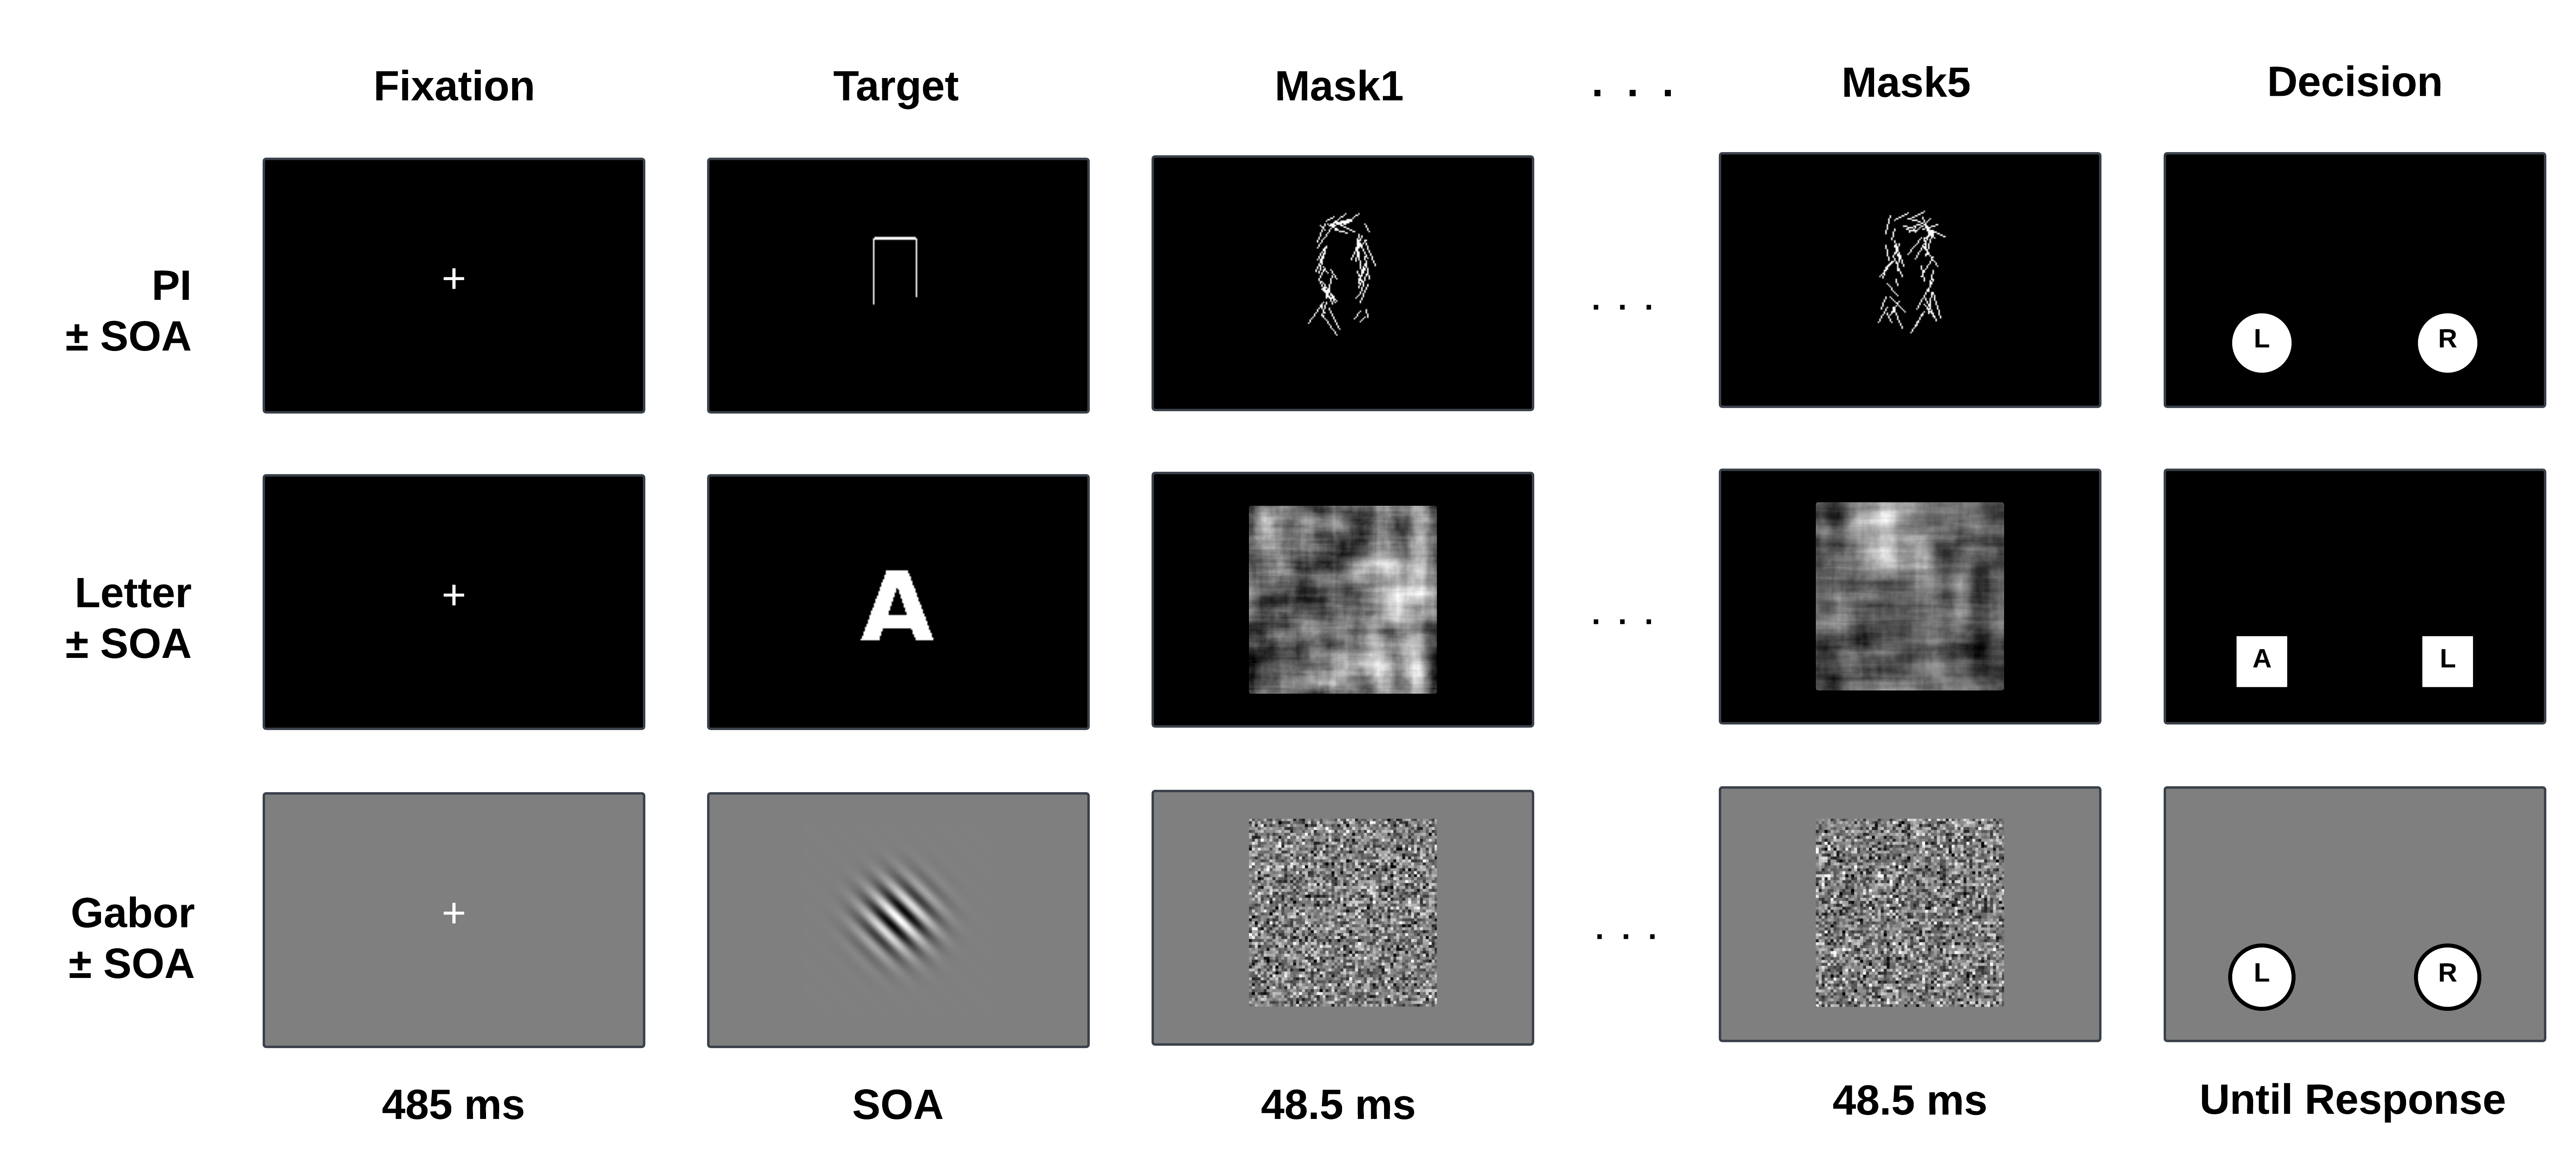
\includegraphics[width=1\linewidth]{Figures/Temporal} \caption{Backward visual masking tasks.}\label{fig:backward}
\end{figure}

\begin{figure}
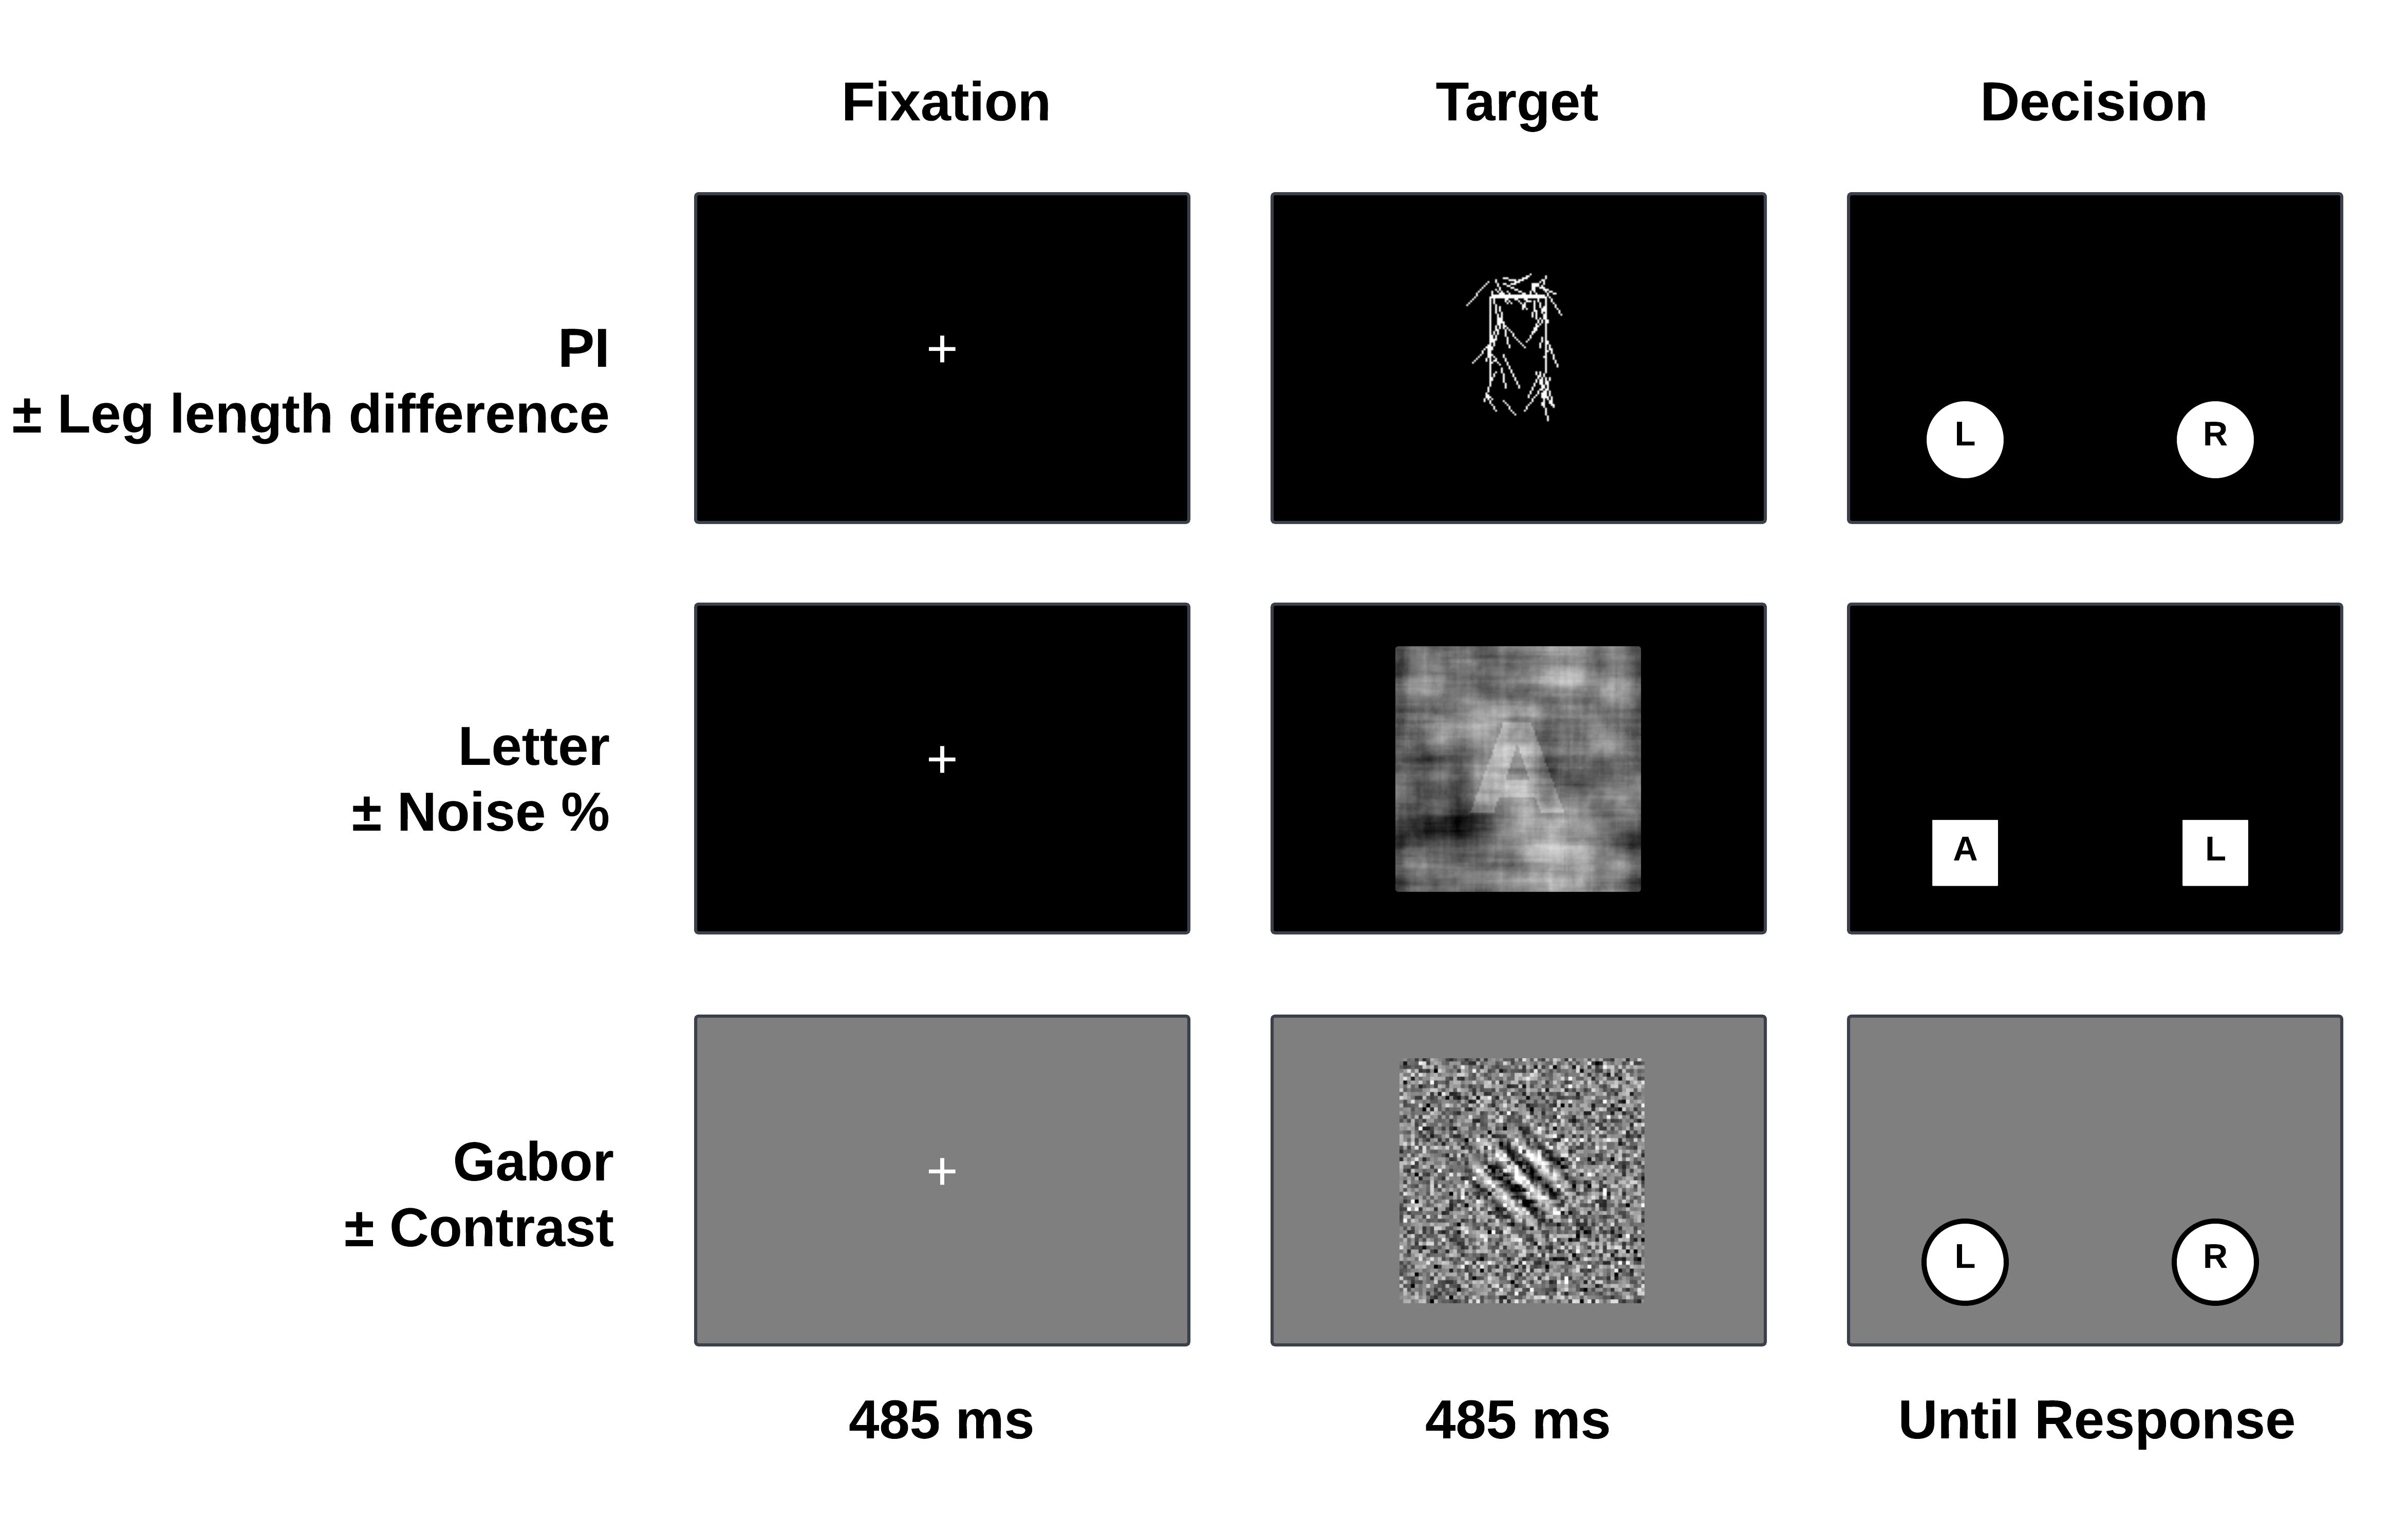
\includegraphics[width=1\linewidth]{Figures/Spatial} \caption{Simultaneous visual masking tasks.}\label{fig:simultaneous}
\end{figure}

\begin{figure}
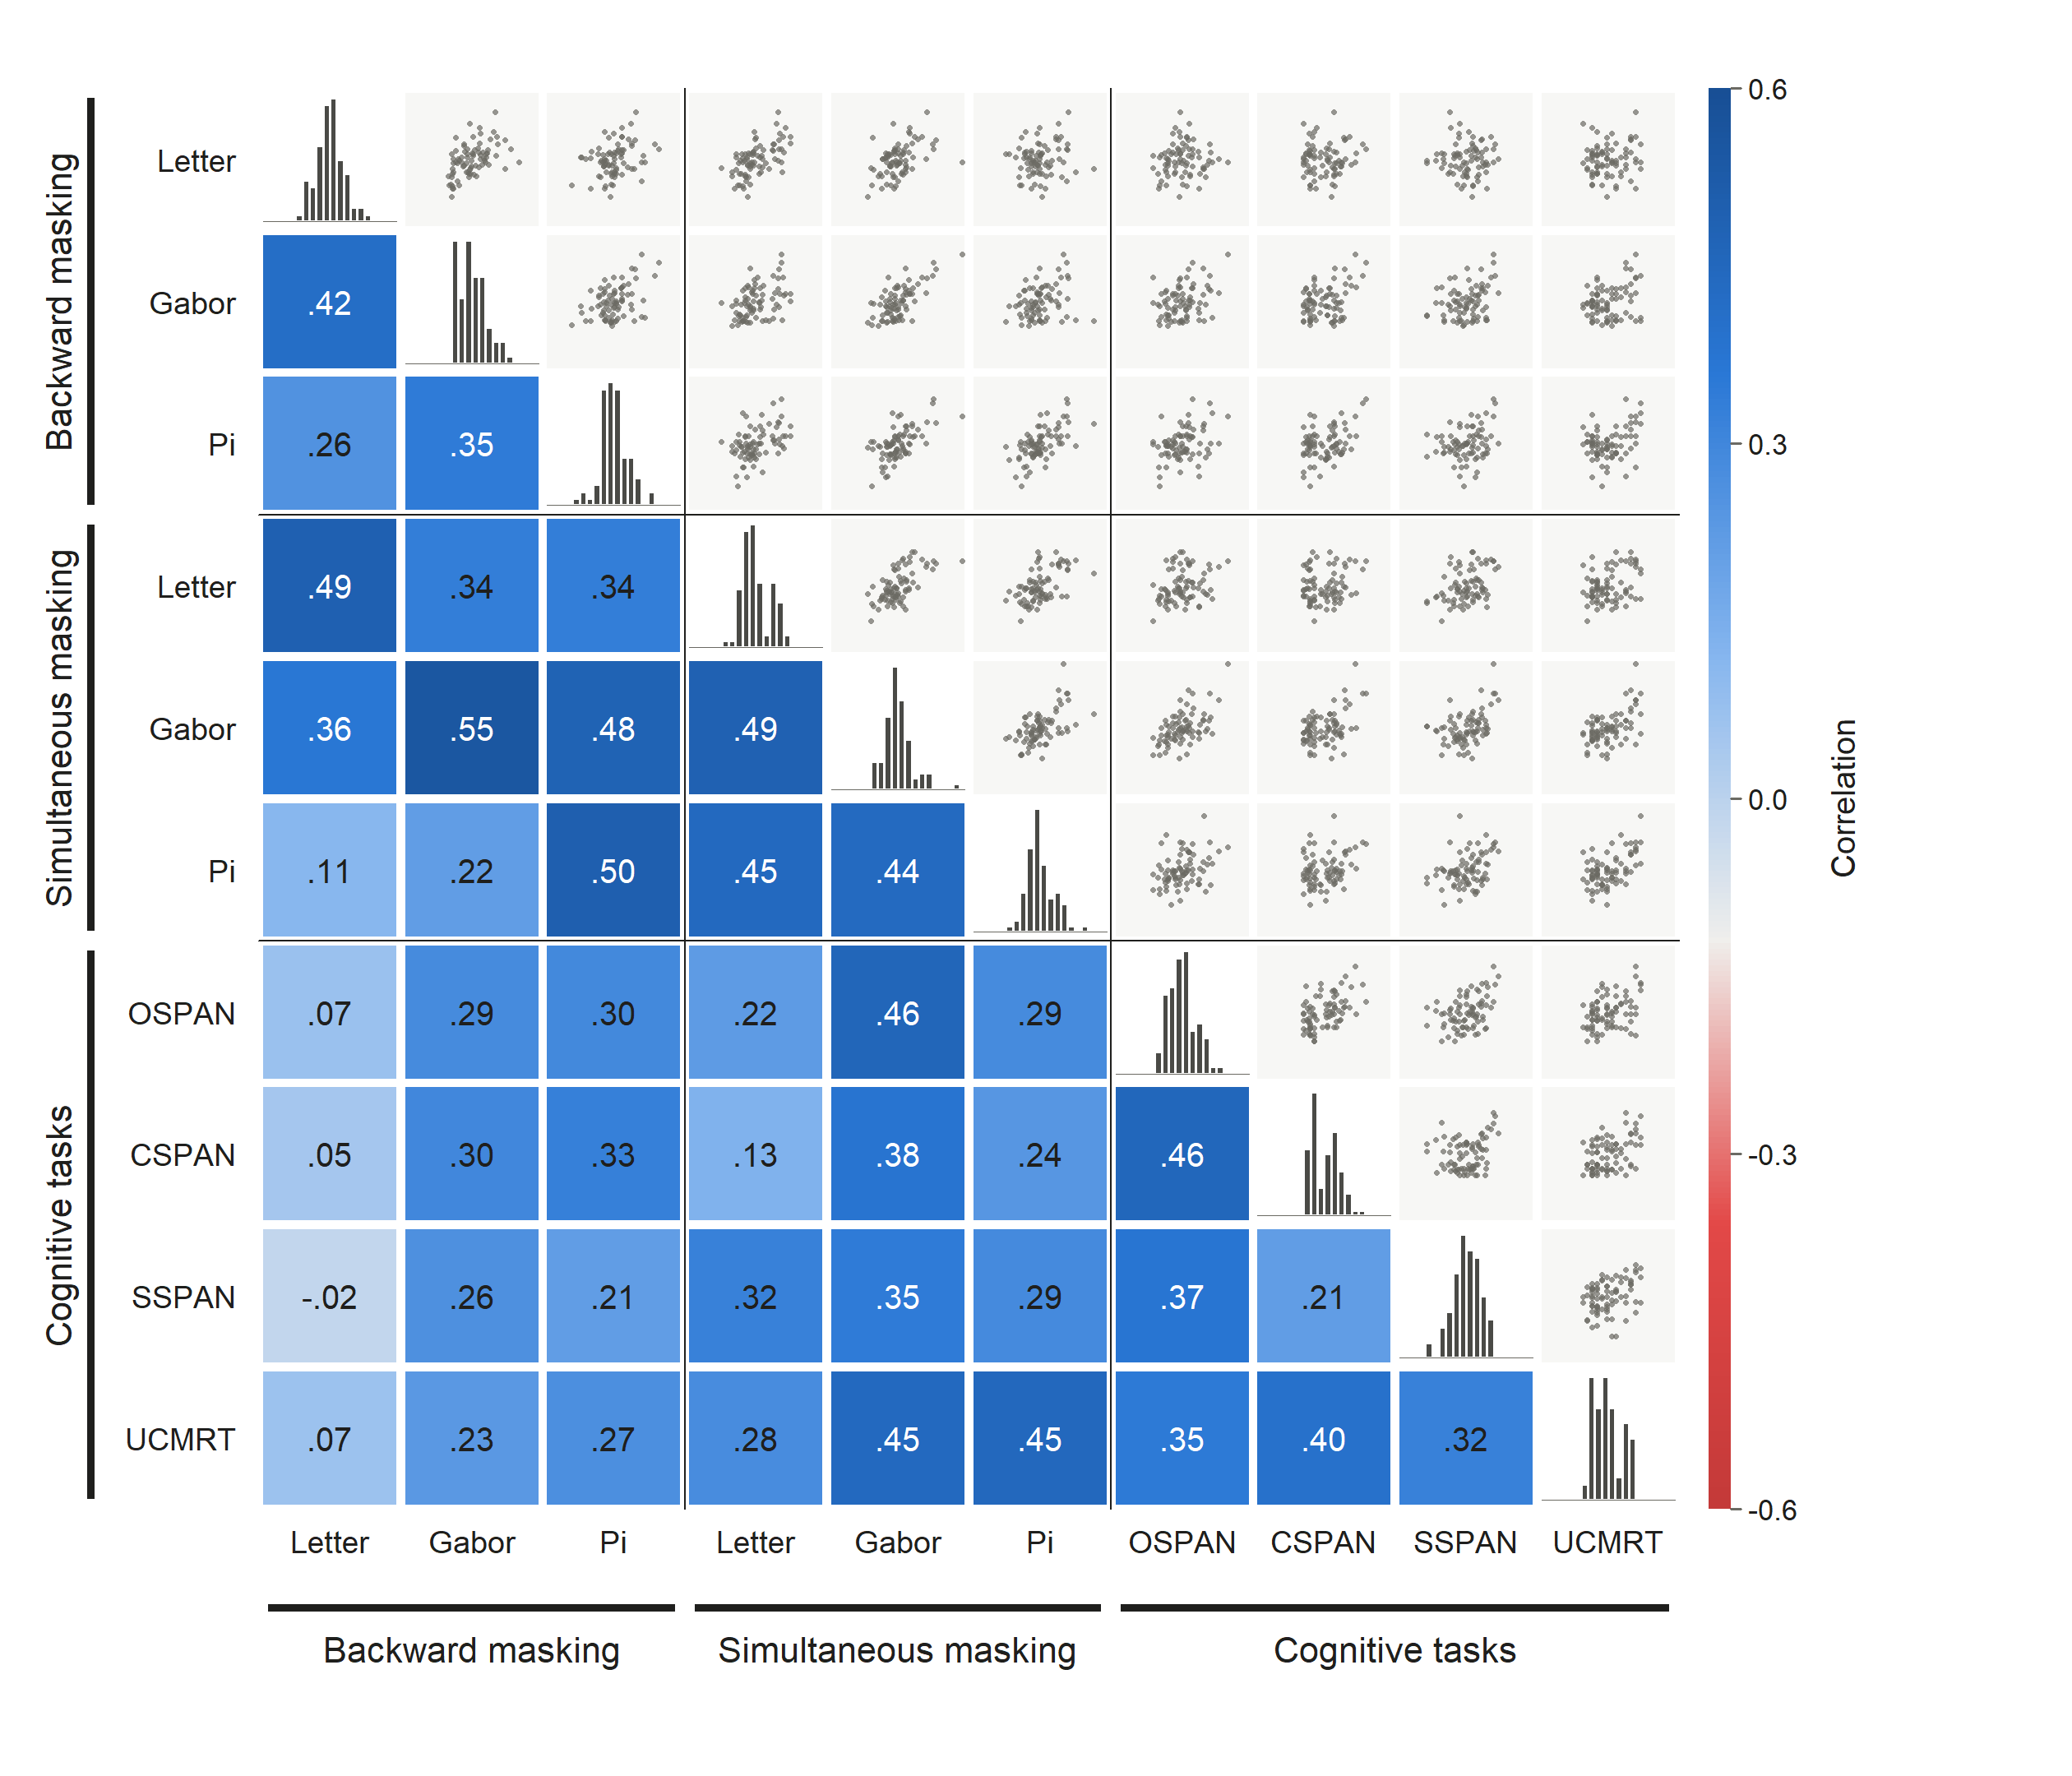
\includegraphics[width=1\linewidth]{Figures/corr} \caption{Model-estimated scores and correlations for the six masking tasks and the four cognitive tasks. Diagonal: distributions of the standardized scores. Lower triangle: model-estimated correlations. Upper triangle: scatterplots of the standardized scores.}\label{fig:corr}
\end{figure}

\begin{figure}
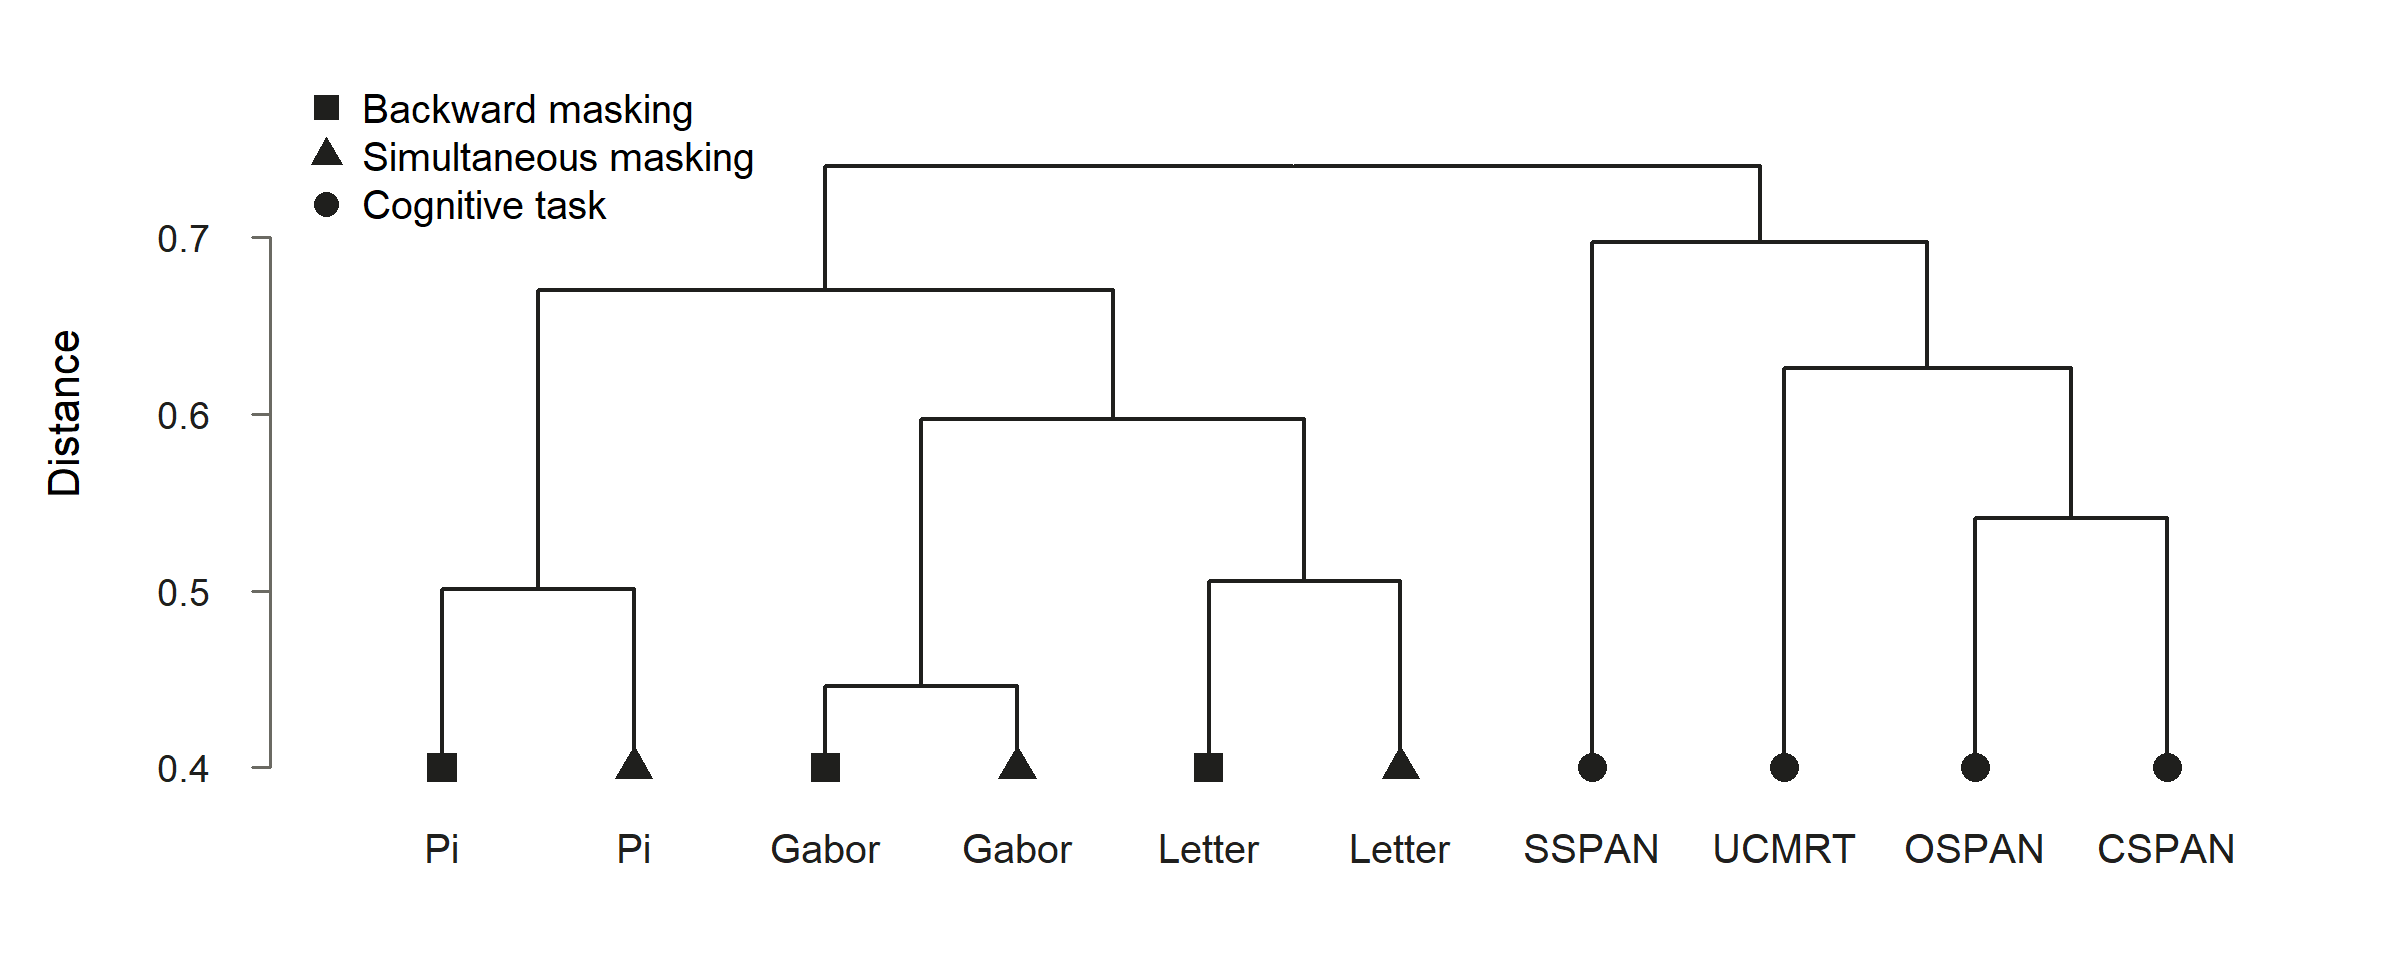
\includegraphics[width=1\linewidth]{Figures/hcluster} \caption{Hierarchical clustering of the ten tasks, based on the distance $1 - r$ between model-estimated correlations and average linkage. Symbols mark backward masking, simultaneous masking, and cognitive tasks.}\label{fig:hcluster}
\end{figure}

\section{Introduction}\label{introduction}

Understanding how fundamental perceptual abilities interrelate and contribute to cognitive performance is one of the central topics in cognitive psychology and individual-differences research. Perhaps the best-known finding in this literature concerns inspection time (IT), the minimum exposure duration at which an observer can reliably make a simple perceptual discrimination. Vickers, Nettelbeck, and Willson (1972) first introduced this paradigm. In its classic form, participants briefly view a stimulus consisting of two vertical lines of clearly unequal length joined at the top (hereafter, the Pi stimulus) and indicate which line is longer. By varying the exposure duration of the Pi stimulus and using a backward mask to prevent further visual processing, the minimum exposure duration required for accurate discrimination can be estimated. Nettelbeck and Lally (1976) subsequently reported that IT correlated negatively with Performance IQ. This negative relation has since been replicated many times across age groups, sensory modalities, and measures of intelligence (Deary, Caryl, Egan, \& Wight, 1989; Deary \& Stough, 1996; Osmon \& Jackson, 2002). Meta-analyses place the uncorrected correlation between IT and intelligence at about -.3, rising to about -.5 after correction for measurement error and range restriction (Grudnik \& Kranzler, 2001; Kranzler \& Jensen, 1989). The standard interpretation of this association is in terms of \emph{processing speed}. Because the mask interrupts further processing of the target, performance depends on how much target information the observer can extract before the mask arrives; individuals who process information faster therefore require shorter exposures to discriminate the stimulus accurately (Vickers \& Smith, 1986). Faster information processing, in turn, may benefit cognitive performance across a wide range of tasks (Vernon, 1983), resulting in negative correlations between IT and cognitive performance.

\emph{Backward masking} is therefore a key manipulation for limiting how much target information can be extracted. As the interval between target onset and mask onset shortens, only observers who process information quickly can extract enough information from the target before the mask disrupts further processing. The situation changes, however, when target and mask are presented at the same time and remain on the screen for a sufficient duration. The target is then embedded in the mask rather than interrupted by it, a procedure known as \emph{simultaneous masking}. In simultaneous masking, processing time is no longer the limiting factor; performance instead depends on how precisely the relevant features of the target can be extracted from the concurrent noise. This taps the same sensory discrimination ability assessed by classic sensory discrimination tasks, in which observers judge which of two stimuli is higher in pitch or longer in length (Deary, 1994b; Deary, Bell, Bell, Campbell, \& Fazal, 2004). In both cases, performance is limited by how precisely the signal is represented relative to noise, whether that noise is added to the display or arises within the sensory system (Pelli \& Farell, 1999). We therefore treat simultaneous masking as a measure of sensory discrimination and use this term throughout the remainder of the paper.

Sensory discrimination, like processing speed, has long been linked to cognitive performance. Galton (1883) proposed that finer sensory acuity supplies the raw material for intelligent judgment, and Spearman (1904) found that discrimination of pitch, light, and weight loaded on a general factor of intelligence, which he termed \emph{g}. Subsequent studies have reported reliable correlations between single discrimination tasks and intelligence (Mikellidou, Lambrou, Georgiou, \& Avraamides, 2023; Mosing, Pedersen, Madison, \& Ullén, 2014; Raz, Willerman, \& Yama, 1987). Deary et al. (2004) reported a latent correlation of .92 between general discrimination and general intelligence.

Although both processing speed and sensory discrimination have shown reliable correlations with cognitive performance, few studies have measured them in the same participants, and none, to our knowledge, has done so with the same stimuli and masks. The closest precedent is Tsukahara, Harrison, Draheim, Martin, and Engle (2020), which measured both constructs in the same participants. However, their sensory discrimination tasks required auditory judgments of the pitch, loudness, or duration of tones, whereas their processing speed tasks required speeded comparisons of visually presented letter and digit strings. When stimulus, sensory modality, and construct vary together, two alternative interpretations cannot be ruled out. First, individual differences may be partly stimulus-specific. Studies that administer batteries of visual tasks to the same observers typically find weak correlations among tasks (Cappe, Clarke, Mohr, \& Herzog, 2014; Tulver, 2019), so an observer may perform well with one type of stimulus but poorly with another. An apparent dissociation between processing speed and sensory discrimination may then reflect differences between the materials rather than between the processes. Second, the variance that the two kinds of tasks share may reflect a general perceptual factor rather than two distinct abilities (Deary, 1994a), in which case the distinction between sensory discrimination and processing speed would not hold at the level of individual differences. In the present study, we addressed both possibilities by holding the stimulus constant while varying only the masking procedure. We used three stimulus types, a Gabor patch, a letter, and the Pi stimulus, and each was presented with an identical mask under both backward masking and simultaneous masking. This fully crossed 2 (masking procedure) × 3 (stimulus type) design follows the logic of the multitrait--multimethod matrix (Campbell \& Fiske, 1959): because every stimulus appears under both masking procedures, variance associated with the masking procedure can be separated from variance associated with the stimulus. If sensory discrimination and processing speed are distinct abilities, tasks that share a masking procedure should correlate more strongly than tasks that share a stimulus; if individual differences are instead organized by stimulus content, the reverse should hold.

Participants also completed three complex span tasks of working memory (Conway et al., 2005; Pahor, Seitz, \& Jaeggi, 2022; Unsworth, Heitz, Schrock, \& Engle, 2005) and a matrix reasoning test of fluid intelligence (Pahor, Stavropoulos, Jaeggi, \& Seitz, 2019), which together served as our measures of cognitive performance. This allowed us to ask, in addition, whether sensory discrimination and processing speed share their relation to cognitive performance, and whether that relation depends on stimulus content.

\section{Method}\label{method}

\subsection{Participants}\label{participants}

Eighty-three undergraduate students at the University of California, Irvine, participated in exchange for \$50 in total compensation. Four participants withdrew before completing all sessions, leaving a final sample of 79. All participants reported normal or corrected-to-normal vision and provided informed consent. The study was approved by the Institutional Review Board of the University of California, Irvine (Study ID: STUDY00000064).

\subsection{Apparatus}\label{apparatus}

Participants were tested individually in a dimly lit cubicle, seated approximately 100 cm from a 24-inch BenQ LED gaming monitor (1920 × 1080 pixels, 165 Hz refresh rate, 6.06 ms per frame). Stimuli were generated with PsychoPy3 (Peirce et al., 2019) in Python 3.8, running on a PC with Lubuntu Linux 22.04. The background was a uniform mid-gray with a luminance of approximately 100 cd/m².

\subsection{Tasks}\label{tasks}

To assess the sensory discrimination ability and processing speed, the experiment contained six visual masking tasks: three employing backward masking (Figure \ref{fig:backward}) and three employing simultaneous masking (Figure \ref{fig:simultaneous}). Both sets of tasks used the same stimulus classes (a Gabor stimulus, a letter stimulus, and a Pi stimulus) and mask classes. The critical difference was the masking procedure: in the backward masking tasks, the mask followed the stimulus after a variable stimulus--onset asynchrony (SOA), whereas in the simultaneous masking the stimulus and mask were presented simultaneously.

To assess cognitive performance, participants completed three complex span tasks of working memory (OSPAN, CSPAN, and SSPAN) and one matrix reasoning test of fluid intelligence (UCMRT). Because working memory capacity and fluid intelligence are strongly related constructs (Kane, Hambrick, \& Conway, 2005), and because our main goal was to examine how sensory discrimination and processing speed relate to cognitive performance as a whole rather than to its specific components, we treated the four tasks as joint indicators of a single construct, which we refer to as \emph{cognitive performance}.

\subsubsection{Sensory discrimination tasks}\label{sensory-discrimination-tasks}

\textbf{Gabor.}\(\quad\)Participants completed a two-alternative forced-choice orientation discrimination task. On each trial, a fixation cross was presented for 485 ms, followed by a centrally presented, random-phase Gabor patch (±45° orientation) embedded in white noise, which remained on the screen for another 485 ms. Participants indicated whether the grating was tilted up-left or up-right by pressing the keyboard. Task difficulty was adaptively adjusted by varying stimulus contrast.

\textbf{Letter.}\(\quad\)Participants performed a forced-choice letter identification task using the keys A--L (second keyboard row). Each trial began with a 485 ms fixation cross, followed by a centrally presented target letter (one of A, S, D, F, G, H, J, K, L) displayed for 485 ms. The letter was embedded in a frequency-matched letter noise mask constructed as follows: We constructed the mask by first computing the pixelwise average of the nine possible letters and then perturbing its Fourier spectrum with complex Gaussian noise. After inverse transformation and normalization, this yielded a structured noise pattern with the same overall spatial frequency profile as the average letter image. On each trial, the target letter was linearly blended with this mask, and participants identified the letter using the corresponding keyboard key. Task difficulty was adaptively adjusted by varying the target weight in the letter--noise blend.

\textbf{Pi.}\(\quad\)Participants performed a forced-choice judgment on a \(\Pi\)-shaped (Pi) target, indicating which vertical ``leg'' was longer (left vs.~right). Each trial began with a 485 ms fixation cross, followed by a centrally presented \(\Pi\) stimulus for 485 ms. The mask was composed of random oblique line segments arranged to form a \(\Pi\)-like clutter. Short line elements (randomized in length and orientation within ±10°--45°) were placed in two vertical columns aligned with the legs of the \(\Pi\) and around the crossbar region. Equal numbers of lines were drawn on each side, although their random placement could introduce local asymmetries. On each trial, the target \(\Pi\) was superimposed on this cluttered mask, and participants indicated which leg appeared longer using the keyboard. Task difficulty was adaptively controlled by varying the leg-length difference.

\subsubsection{Processing speed tasks}\label{processing-speed-tasks}

\textbf{Gabor.}\(\quad\)The task matched the simultaneous Gabor-orientation discrimination task. Each trial began with a 485 ms fixation cross, followed by a centrally presented, random-phase Gabor patch (±45° orientation). After a variable SOA, the target was replaced by a dynamic sequence of five white noise masks (48.5 ms each). Participants indicated whether the grating was tilted up-left or up-right by pressing the keyboard. Task difficulty was adaptively adjusted by SOA.

\textbf{Letter.}\(\quad\)The task matched the simultaneous letter-identification condition. Each trial began with a 485 ms fixation cross, followed by a centrally presented target letter (one of A, S, D, F, G, H, J, K, L). After a variable SOA, the target was replaced by a dynamic sequence of five frequency-matched letter noise masks (48.5 ms each). Participants identified the letter using the corresponding keyboard key. Task difficulty was adaptively adjusted by varying SOA.

\textbf{Pi.}\(\quad\)The task matched the simultaneous \(\Pi\)-leg discrimination condition. Each trial began with a 485 ms fixation cross, followed by a centrally presented \(\Pi\) stimulus. After a variable SOA, the target was replaced by a dynamic sequence of five clutter masks composed of randomly oriented oblique line segments (48.5 ms each). Participants indicated which leg appeared longer using the keyboard. Task difficulty was adaptively controlled by varying SOA.

\subsubsection{Cognitive tasks}\label{cognitive-tasks}

\textbf{OSPAN.}\(\quad\)Participants completed an automated OSPAN task (Unsworth et al., 2005) combining simple math operations with working memory recall for letter sequence. Each set contained 3--7 letters, with each set size presented three times, yielding 15 memory sets in total. Before the main task, participants completed three practice sets of size three to familiarize themselves with the procedure. In the main task, set sizes 3--7 were each presented three times in randomized order (15 sets total). Within each set, trials alternated between (i) a math operation screen (e.g., ``6 + 2 = ?''), after which the participant clicked to continue, and (ii) a proposed answer screen showing a single digit; participants judged whether the digit correctly solved the operation by clicking true/false. A single uppercase letter was then shown for 800 ms, and the sequence continued until the set ended. At recall, participants clicked the letters in serial order from a matrix. For each set, participants earned points equal to the set size only if (a) all math operations were solved within the participant's mean solving time in the practice trials plus 2.5 SD, (b) no math errors occurred for that set, and (c) all letters were recalled in the correct order. Sets failing any criterion scored 0. The final OSPAN score was the sum of points across all sets.

\textbf{CSPAN.}\(\quad\)Participants completed a CSPAN task (Conway et al., 2005) combining serial counting with working memory recall for number sequence. Each display contained a set of target items (green circles) intermixed with distractors (yellow circles). Participants counted the number of targets in each display, after which the participant clicked to continue to the next display. At recall, participants were prompted to recall the sequence of counts (e.g., ``3--5--2'') in the exact order they were encountered. Responses were made by clicking the digits from a matrix. The procedure began with three practice sets of size 2. The main task then presented set sizes 3--7, each three times in randomized order (15 sets total). A set contributed points equal to its size only if the final recall sequence was accurate in both values and order. The final CSPAN score was the sum of points across all sets.

\textbf{SSPAN.}\(\quad\)Participants completed a SSPAN task adapted from the Corsi block-tapping paradigm to assess both storage and processing aspects of spatial working memory (Pahor et al., 2022). On each trial, cartoon gophers appeared sequentially in one of 12 possible screen locations, each presented for 1,500 ms with a 500 ms inter-stimulus interval. Participants were required to reproduce the sequence by tapping the corresponding locations in the exact order. Between each gopher presentation participants performed a secondary sorting task, dragging an item to the left or right, thereby imposing concurrent processing demands and limiting reliance on mnemonic strategies. Sequence length ranged adaptively from 2 to 10 items, increasing or decreasing in difficulty depending on accuracy. The final SSPAN score was the total successfully recalled items across all sets.

\textbf{UCMRT.}\(\quad\)Participants completed the UCMRT (Pahor et al., 2019), a measure of fluid intelligence modeled after Raven's Progressive Matrices. Each trial presented a 3×3 matrix of abstract visual patterns with the bottom-right cell missing, and participants selected the option that best completed the matrix from eight alternatives displayed below. UCMRT was chosen because it was especially developed for young adults with above-average performance on matrix reasoning tasks, providing a more sensitive and efficient assessment of individual differences in fluid intelligence in this population. The task consisted of 23 problems of varying difficulty, including 2 two-relation items, 3 three-relation items with a single transformation, 6 three-relation items with two transformations, 6 three-relation items with three transformations, and 6 logic items. Performance was scored as accuracy, defined by the number of correctly solved matrices.

\subsection{Procedure}\label{procedure}

The experiment consisted of three sessions of approximately one hour each, conducted on separate days within one week. Each session comprised three blocks, with short breaks permitted between blocks. The first and third blocks were visual masking blocks, and the middle block contained the cognitive tasks for that session: OSPAN on the first day, CSPAN on the second day, SSPAN task and the UCMRT on the third day.

Within each visual masking block, participants completed all six visual masking tasks in random order. Each task consisted of 50 trials, on which a two-down--one-up and a three-down--one-up staircase strictly alternated, yielding 25 trials per staircase. Because the two staircases converge on different performance levels, approximately 70.7\% and 79.4\% correct, respectively (Levitt, 1971), alternating them allowed the psychometric function to be estimated more precisely. In total, each participant completed 300 trials per task (6 blocks × 50 trials). The first masking block served as practice and was excluded from analysis, leaving 250 trials per task (125 per staircase) and 1,500 masking trials per participant for analysis.

\subsection{Data exclusion}\label{data-exclusion}

Data were screened separately for each participant and each masking task. A participant's data on a given task were excluded from further analysis if either of two criteria was met. First, the participant's raw threshold, computed as the mean stimulus level across the 250 analyzed trials, deviated by more than four standard deviations from the group mean threshold for that task. Second, the observed accuracy on either staircase deviated by more than 5 percentage points from its target accuracy (70.7\% for the two-down--one-up staircase and 79.4\% for the three-down--one-up staircase), indicating that the staircase had not converged as intended. In total, 14 task datasets from 10 participants were excluded. These participants' remaining tasks were retained in the analysis.

\subsection{Hierarchical psychometric model}\label{hierarchical-psychometric-model}

Individual thresholds on the masking tasks and the correlations among them were estimated with a hierarchical psychometric model (Rouder \& Mehrvarz, 2026). The model estimates individual thresholds and their correlations simultaneously from trial-level data, thereby accounting for trial-to-trial noise and avoiding the attenuation of correlations caused by measurement error.

At the data level, let \(y_{ijk}\) denote the binary correctness outcome on the \(k\)-th trial of participant \(i\) in task \(j\). We assume
\[
y_{ijk} \sim \text{Bernoulli}\!\left(F(s_{ijk}; \theta_{ij}, \beta_{j})\right),
\]

where the success probability is given by a task-specific psychometric function, modeled as a cumulative normal function of log stimulus strength with a lower asymptote at chance:

\[
F(s_{ijk}; \theta_{ij}, \beta_{j}) = \gamma_j + (1-\gamma_j)\,\Phi\!\left(\beta_j\,(s_{ijk}-\theta_{ij})\right).
\]

Here, \(\Phi(\cdot)\) denotes the standard normal cumulative distribution function, and \(\gamma_j\) is the guessing rate for task \(j\), fixed at .5 for the two-alternative Gabor and Pi tasks and at 1/9 for the nine-alternative Letter tasks. The variable \(s_{ijk}\) denotes the stimulus strength on trial \(k\) for participant \(i\) on task \(j\), log-transformed and then standardized within each task. In the backward masking tasks, stimulus strength was the SOA; in the simultaneous masking tasks, it was the Gabor contrast, the target weight in the letter--noise blend, and the leg-length difference of the Pi stimulus, respectively. The parameter \(\theta_{ij}\) denotes the latent threshold of participant \(i\) on task \(j\), expressed on the same scale as \(s_{ijk}\), and \(\beta_j\) denotes the slope of the psychometric function for task \(j\).

At the latent level, each participant is characterized by a vector of ten person-level parameters: the six latent thresholds from the masking tasks and the standardized scores on the four cognitive tasks,

\[
\boldsymbol{\theta}_i = \left(\theta_{i1}, \ldots, \theta_{i6}, c_{i1}, \ldots, c_{i4}\right)^\top,
\]

where \(c_{im}\) denotes the standardized score of participant \(i\) on cognitive task \(m\). These ten parameters are assumed to follow a multivariate normal distribution,

\[
\boldsymbol{\theta}_i \sim \mathcal{N}_{10}\!\left(\boldsymbol{\mu}, \boldsymbol{\Sigma}\right),
\]

where \(\boldsymbol{\mu}\) captures the mean of each task and \(\boldsymbol{\Sigma}\) captures the covariance among tasks. The covariance matrix is given a scaled inverse-Wishart (SIW) prior (Huang \& Wand, 2013) which is robust to differences in the measurement scales of the tasks and is computationally efficient to estimate (Yang \& Rouder, 2026). Full details of the model specification are provided in Appendix A.

\section{Results}\label{results}

\subsection{Individual differences and their correlational structure}\label{individual-differences-and-their-correlational-structure}

Figure \ref{fig:corr} summarizes the model-estimated scores for the six masking tasks and the four cognitive tasks. All scores were standardized before plotting. The distributions on the diagonal were unimodal and roughly symmetric, with substantial spread across participants. Thus, all ten tasks captured meaningful individual differences. The lower triangle of Figure \ref{fig:corr} shows the model-estimated correlations among the ten tasks. All 45 correlations were positive with a single exception between the backward Letter task and SSPAN (\emph{r} = -.02). The mean correlation was .39 among the six masking tasks, .35 among the four cognitive tasks, and .26 between the masking tasks and the cognitive tasks.

It is worth noting that the three same-stimulus pairs, in which the same stimulus was tested under backward and simultaneous masking, showed the three highest correlations among the masking tasks (mean \emph{r} = .52). By comparison, the mean correlation was .40 between tasks that shared a masking procedure but differed in stimulus, and .31 between tasks that differed in both. This pattern suggests that stimulus type plays a substantial role in individual differences in masking performance. More direct evidence comes from hierarchical clustering, an unsupervised method that groups tasks according to their similarity without imposing any a priori structure (see Figure \ref{fig:hcluster}). The first three merges each joined the two masking procedures of the same stimulus; only after these pairs had formed did they combine with one another. By comparison, neither the three backward masking tasks nor the three simultaneous masking tasks formed a cluster of their own. The four cognitive tasks formed a separate cluster, which joined the masking tasks only at the final step. Thus, individual differences in masking performance were organized primarily by stimulus rather than by masking procedure.

\subsection{Structural decomposition of masking performance}\label{structural-decomposition-of-masking-performance}

Hierarchical clustering showed that the structure among the masking tasks is best described by grouping by stimulus type. The next question is whether stimulus type or masking procedure contributes to cognitive performance. These two questions are different because the covariance that determines how tasks cluster need not be the covariance that predicts cognitive performance. Tasks sharing a stimulus may cluster together because of stimulus-specific variance, while their relation to cognitive performance may instead be carried by other sources of variance, for example, variance from the masking procedure or variance from a common visual factor.

To answer this question, we retained the data level of the hierarchical psychometric model and replaced the covariance matrix \(\boldsymbol{\Sigma}\) at the latent level with a structural equation model. For the six masking tasks, the thresholds \(\theta_{ij}\) remain linked to the trial-level data through the psychometric function \(F(s_{ijk}; \theta_{ij}, \beta_j)\); what changes is how the person-level vector \(\boldsymbol{\theta}_i\) is generated. In the new latent structure, \(\boldsymbol{\theta}_i\) is expressed as a function of seven latent factors,

\[
\boldsymbol{\eta}_i = \left(\eta_i^{V}, \eta_i^{\text{Bwd}}, \eta_i^{\text{Sim}}, \eta_i^{\text{Let}}, \eta_i^{\text{Gab}}, \eta_i^{\text{Pi}}, \eta_i^{C}\right)^\top,
\]

where \(\eta_i^{V}\) is a general visual factor shared by all six masking tasks; \(\eta_i^{\text{Bwd}}\) and \(\eta_i^{\text{Sim}}\) are masking factors, each shared by the three tasks that use the same masking procedure; \(\eta_i^{\text{Let}}\), \(\eta_i^{\text{Gab}}\), and \(\eta_i^{\text{Pi}}\) are stimulus factors, each shared by the two tasks that use the same stimulus; and \(\eta_i^{C}\) is a cognitive factor measured by the four cognitive tasks. We refer to the six factors other than \(\eta_i^{C}\) collectively as non-cognitive factors.

The measurement model relates the ten person-level parameters to these factors,

\[
\boldsymbol{\theta}_i = \boldsymbol{\mu} + \boldsymbol{\Lambda}\,\boldsymbol{\eta}_i + \boldsymbol{\epsilon}_i, \qquad
\boldsymbol{\epsilon}_i \sim \mathcal{N}_{10}\!\left(\mathbf{0}, \boldsymbol{\Delta}\right), \qquad
\boldsymbol{\Delta} = \operatorname{diag}\!\left(\delta_1^2, \ldots, \delta_{10}^2\right),
\]

where \(\boldsymbol{\Lambda}\) is a \(10 \times 7\) matrix of factor loadings and \(\delta_j^2\) is the variance unique to task \(j\). With the rows of \(\boldsymbol{\Lambda}\) ordered as in \(\boldsymbol{\theta}_i\) (backward Letter, Gabor, and Pi; simultaneous Letter, Gabor, and Pi; OSPAN, CSPAN, SSPAN, and UCMRT) and the columns ordered as in \(\boldsymbol{\eta}_i\),

\[
\boldsymbol{\Lambda} =
\begin{pmatrix}
\lambda_1^{V} & \lambda_1^{M} & 0 & \lambda_1^{S} & 0 & 0 & 0\\
\lambda_2^{V} & \lambda_2^{M} & 0 & 0 & \lambda_2^{S} & 0 & 0\\
\lambda_3^{V} & \lambda_3^{M} & 0 & 0 & 0 & \lambda_3^{S} & 0\\
\lambda_4^{V} & 0 & \lambda_4^{M} & \lambda_4^{S} & 0 & 0 & 0\\
\lambda_5^{V} & 0 & \lambda_5^{M} & 0 & \lambda_5^{S} & 0 & 0\\
\lambda_6^{V} & 0 & \lambda_6^{M} & 0 & 0 & \lambda_6^{S} & 0\\
0 & 0 & 0 & 0 & 0 & 0 & \lambda_7^{C}\\
0 & 0 & 0 & 0 & 0 & 0 & \lambda_8^{C}\\
0 & 0 & 0 & 0 & 0 & 0 & \lambda_9^{C}\\
0 & 0 & 0 & 0 & 0 & 0 & \lambda_{10}^{C}
\end{pmatrix}.
\]
Each masking task thus loads on the general visual factor (\(\lambda_j^{V}\)), on the factor for its masking procedure (\(\lambda_j^{M}\)), and on the factor for its stimulus (\(\lambda_j^{S}\)), and each cognitive task \(m = 1, \ldots, 4\) loads on the cognitive factor (\(\lambda_{6+m}^{C}\)). All other loadings are fixed at zero.

The structural model specifies the relations among the factors,

\[
\boldsymbol{\eta}_i = \mathbf{B}\,\boldsymbol{\eta}_i + \boldsymbol{\zeta}_i, \qquad
\boldsymbol{\zeta}_i \sim \mathcal{N}_{7}\!\left(\mathbf{0}, \boldsymbol{\Psi}\right), \qquad
\boldsymbol{\Psi} = \mathbf{I}_7,
\]

where \(\mathbf{B}\) is a \(7 \times 7\) matrix of regression weights among the factors. The cognitive factor is regressed on all six non-cognitive factors:

\[
\mathbf{B} =
\begin{pmatrix}
0 & 0 & 0 & 0 & 0 & 0 & 0\\
0 & 0 & 0 & 0 & 0 & 0 & 0\\
0 & 0 & 0 & 0 & 0 & 0 & 0\\
0 & 0 & 0 & 0 & 0 & 0 & 0\\
0 & 0 & 0 & 0 & 0 & 0 & 0\\
0 & 0 & 0 & 0 & 0 & 0 & 0\\
b_{V} & b_{\text{Bwd}} & b_{\text{Sim}} & b_{\text{Let}} & b_{\text{Gab}} & b_{\text{Pi}} & 0
\end{pmatrix},
\]

so that \(\eta_i^{C} = b_{V}\eta_i^{V} + b_{\text{Bwd}}\eta_i^{\text{Bwd}} + b_{\text{Sim}}\eta_i^{\text{Sim}} + b_{\text{Let}}\eta_i^{\text{Let}} + b_{\text{Gab}}\eta_i^{\text{Gab}} + b_{\text{Pi}}\eta_i^{\text{Pi}} + \zeta_i^{C}\). Setting \(\boldsymbol{\Psi} = \mathbf{I}_7\) fixes the variances of the six non-cognitive factors and of the residual \(\zeta_i^{C}\) to one and makes the six non-cognitive factors mutually orthogonal. Because the non-cognitive factors are orthogonal and have unit variance, this structure separates the two questions raised above. First, the variance of each masking task decomposes additively,

\[
\operatorname{Var}(\theta_{ij}) = \left(\lambda_j^{V}\right)^2 + \left(\lambda_j^{M}\right)^2 + \left(\lambda_j^{S}\right)^2 + \delta_j^2,
\]

so the proportion of variance due to each source is its term divided by \(\operatorname{Var}(\theta_{ij})\). Second, the relation of each non-cognitive factor \(f \in \{V, \text{Bwd}, \text{Sim}, \text{Let}, \text{Gab}, \text{Pi}\}\) to cognitive performance is captured by its regression weight \(b_f\), and the corresponding correlation \(r_f\) is

\[
\operatorname{Var}\!\left(\eta_i^{C}\right) = \sum_f b_f^2 + 1, \qquad
r_f = \frac{b_f}{\sqrt{\operatorname{Var}\!\left(\eta_i^{C}\right)}}.
\]
Full details of the model specification are provided in Appendix B. Derivations of the variance decomposition are provided in Appendix C.

\subsubsection{Sources of variance in masking performance}\label{sources-of-variance-in-masking-performance}

Table \ref{tab:tab-shares} shows how the variance of each masking task was distributed across the general visual factor, the masking factors, the stimulus factors, and task-unique variance. The general visual factor was the largest shared source of variance. It accounted for 32\% of the variance on average. The stimulus factors were the second largest shared source, accounting for 18\% of the variance on average. The masking factors accounted for the smallest share, 11\% of the variance on average. The remaining 40\% of the variance was unique to each task.

\begin{table}[tbp]

\begin{center}
\begin{threeparttable}

\caption{\label{tab:tab-shares}Proportion of variance of each masking task due to each source.}

\begin{tabular}{lcccc}
\toprule
Task & \multicolumn{1}{c}{General} & \multicolumn{1}{c}{Masking} & \multicolumn{1}{c}{Stimulus} & \multicolumn{1}{c}{Unique}\\
\midrule
Backward Letter & .19 [.01, .46] & .14 [.00, .42] & .23 [.01, .53] & .44 [.21, .71]\\
Backward Gabor & .28 [.04, .57] & .14 [.00, .44] & .19 [.00, .52] & .39 [.16, .68]\\
Backward Pi & .38 [.11, .66] & .05 [.00, .22] & .18 [.00, .50] & .39 [.18, .65]\\
Simultaneous Letter & .34 [.09, .60] & .10 [.00, .34] & .16 [.00, .40] & .41 [.21, .66]\\
Simultaneous Gabor & .41 [.14, .65] & .06 [.00, .23] & .09 [.00, .29] & .45 [.27, .66]\\
Simultaneous Pi & .33 [.05, .67] & .15 [.00, .49] & .20 [.00, .54] & .31 [.11, .60]\\
\textbf{Average} & \textbf{.32 [.20, .45]} & \textbf{.11 [.03, .20]} & \textbf{.18 [.08, .29]} & \textbf{.40 [.30, .51]}\\
\bottomrule
\end{tabular}

\end{threeparttable}
\end{center}

\end{table}

The decomposition shows two results: first, masking-specific variance was small, accounting for roughly a third of the share of the general visual factor. Backward and simultaneous masking were thus largely held together by the general visual factor rather than forming distinct sources of individual differences. Second, stimulus-specific variance tended to be larger than masking-specific variance (posterior probability = .84), in line with the clustering by stimulus reported above.

\subsubsection{Contributions to cognitive performance}\label{contributions-to-cognitive-performance}

Table \ref{tab:tab-cor} shows the correlation of each non-cognitive factor with cognitive performance. Bayes factors are Savage--Dickey density ratios. We interpreted them following Kass and Raftery (1995): \(\text{BF}_{10}\) values above 3 provide positive evidence for a relation, and values above 20 provide strong evidence. Only the general visual factor was reliably related to cognitive performance, \(r = .58\), 95\% CI {[}.22, .82{]}, and the Bayes factor provided strong evidence for this relation, \(\text{BF}_{10} = 34.1\).

\begin{table}[tbp]

\begin{center}
\begin{threeparttable}

\caption{\label{tab:tab-cor}Correlation of each non-cognitive factor with cognitive performance.}

\begin{tabular}{lcc}
\toprule
Factor & \multicolumn{1}{c}{$r$} & \multicolumn{1}{c}{$\text{BF}_{10}$}\\
\midrule
General visual factor & .58 [.22, .82] & \textbf{34.1}\\
Backward masking & -.06 [-.46, .38] & 0.50\\
Simultaneous masking & .21 [-.25, .61] & 0.79\\
Letter & -.22 [-.55, .20] & 0.86\\
Gabor & .31 [-.16, .68] & 1.47\\
Pi & .10 [-.29, .48] & 0.53\\
\bottomrule
\addlinespace
\end{tabular}

\begin{tablenotes}[para]
\normalsize{\textit{Note.} $r$ is the posterior mean of the correlation $r_f$ between each non-cognitive factor and the cognitive factor, with 95\% credible interval. Bayes factors are Savage--Dickey density ratios with prior $b_f \sim \mathcal{N}(0, 1)$. $\text{BF}_{10}$ values above 3 provide positive evidence for a relation, and values above 20 provide strong evidence.}
\end{tablenotes}

\end{threeparttable}
\end{center}

\end{table}

None of the specific factors showed a comparable relation. All five credible intervals included zero, and the correlations did not share a common sign. All Bayes factors fell in the inconclusive range. Thus, the data provided no evidence that stimulus-specific or masking-specific variance contributes to cognitive performance.

Taken together, stimulus content accounted for a substantial share of individual differences in masking performance, yet this stimulus-specific variance showed no evidence of a relation to cognitive performance. The relation between masking performance and cognitive performance was instead carried by the general visual factor shared by all six masking tasks.

\section{Discussion}\label{discussion}

We asked whether sensory discrimination and processing speed, as indexed by simultaneous and backward masking of the same stimuli, reflect separable sources of individual differences. Three findings emerged. First, backward and simultaneous masking were largely held together by a general visual factor, which was the largest shared source of variance in the masking tasks; variance specific to the masking procedure was small. Second, there was a clear stimulus effect: tasks that shared a stimulus correlated most strongly, clustered together, and shared stimulus-specific variance beyond the general factor. Third, despite this stimulus effect, only the general visual factor was related to cognitive performance, whereas neither stimulus-specific nor masking-specific variance showed evidence of such a relation. Thus, varying the masking procedure did not reveal distinct abilities, and varying the stimulus introduced substantial variance that was unrelated to cognitive performance.

\subsection{Sensory discrimination and processing speed are largely not separable}\label{sensory-discrimination-and-processing-speed-are-largely-not-separable}

Sensory discrimination and processing speed have been studied in two largely separate literatures, each of which has been taken to reveal a distinct elementary source of cognitive ability (Deary, 1994a). Our design held the stimulus and the mask constant and varied only whether performance was limited by the time available to encode the target (backward masking) or by the spatial overlap of target and mask (simultaneous masking). Under these conditions, the two procedures shared most of their reliable variance through a single general factor, and the variance specific to each procedure was small. If sensory discrimination and processing speed were distinct abilities, the masking factors should have been substantial, however they were not.

\subsection{A stimulus effect that does not reach cognitive performance}\label{a-stimulus-effect-that-does-not-reach-cognitive-performance}

The second finding concerns the role of the stimulus. The novel finding is that this stimulus-specific variance showed no evidence of a relation to cognitive performance.

\subsection{What does the general visual factor reflect?}\label{what-does-the-general-visual-factor-reflect}

\subsection{Methodological implications}\label{methodological-implications}

The present analysis combined a trial-level psychometric model with a structural equation model at the latent level. Thresholds were estimated directly from trial-level responses, so the correlations among tasks were not attenuated by trial-to-trial noise (Rouder \& Mehrvarz, 2026). Placing the factor model at the latent level, rather than fitting it to a matrix of estimated correlations, extended the uncertainty of the thresholds into the variance decomposition and the regression weights. The same approach can be applied whenever abilities are measured with psychophysical thresholds.

\newpage

\section{Appendix A: Hierarchical Psychometric Model With an Unstructured Covariance Matrix}\label{appendix-a-hierarchical-psychometric-model-with-an-unstructured-covariance-matrix}

\textbf{Model Specification.} Let \(i = 1,\dots,I\) denote individuals, \(j \in \{1,2,3,4,5,6\}\) denote six masking tasks, and \(k = 1,\dots,K\) denote trials. Let \(y_{ijk}\) denote the binary correctness outcome on the \(k\)-th trial of participant \(i\) in masking task \(j\). The data level model is then given by
\[
y_{ijk} \sim \text{Bernoulli}\!\left(F(s_{ijk}; \theta_{ij}, \beta_{j})\right),
\]
where the success probability is given by a task-specific psychometric function, modeled as a cumulative normal function of log stimulus strength with a lower asymptote at chance:
\[
F(s_{ijk}; \theta_{ij}, \beta_{j}) = \gamma_j + (1-\gamma_j)\,\Phi\!\left(\beta_j\,(s_{ijk}-\theta_{ij})\right).
\]
Here, \(\Phi(\cdot)\) denotes the standard normal cumulative distribution function, and \(\gamma_j\) is the guessing rate for task \(j\), fixed at .5 for the two-alternative Gabor and Pi tasks and at 1/9 for the nine-alternative Letter tasks. The variable \(s_{ijk}\) denotes the stimulus strength on trial \(k\) for participant \(i\) on task \(j\), which was log-transformed and then standardized across all trials and participants of task \(j\). Standardization places the six masking tasks on a common scale, so that the same priors can be used for all tasks; because it is a linear transformation within each task, it does not affect the correlations among tasks. The parameter \(\theta_{ij}\) denotes the latent threshold of participant \(i\) on task \(j\), expressed on the same scale as \(s_{ijk}\). \(\beta_j\) denotes the slope of the psychometric function for task \(j\).

At the latent level, each participant is characterized by a vector of ten person-level parameters: the six latent thresholds from the masking tasks and the standardized scores on the four cognitive tasks,
\[
\boldsymbol{\theta}_i = \left(\theta_{i1}, \ldots, \theta_{i6}, c_{i1}, \ldots, c_{i4}\right)^\top,
\]
where \(c_{im}\) denotes the standardized score of participant \(i\) on cognitive task \(m\). These ten parameters are assumed to follow a multivariate normal distribution
\[
\boldsymbol{\theta}_i \sim \mathcal{N}_{10}\!\left(\boldsymbol{\mu}, \boldsymbol{\Sigma}\right).
\]
The cognitive scores enter the model as observed values of the last four elements of \(\boldsymbol{\theta}_i\). Specifically, the observed standardized score \(x_{im}\) of participant \(i\) on cognitive task \(m\) is modeled as
\(x_{im} \sim \mathcal{N}(c_{im}, \tau^2)\) with \(\tau = 0.01\), so that \(c_{im}\) is constrained to be essentially equal to the observed score.

\textbf{Prior specification.} Priors are needed for the task means \(\boldsymbol{\mu}\), the slopes \(\beta_j\), and the covariance matrix \(\boldsymbol{\Sigma}\). The task means and slopes were given weakly informative normal priors,
\(\mu_t \sim \mathcal{N}(0, 5^2)\) for \(t = 1, \ldots, 10\) and \(\beta_j \sim \mathcal{N}(0, 5^2)\) for \(j = 1, \ldots, 6\), which are wide relative to the standardized scale of \(s_{ijk}\) and of the cognitive scores. The covariance matrix was given a scaled inverse-Wishart prior (Huang \& Wand, 2013). In this prior, \(\boldsymbol{\Sigma}\) is decomposed into a vector of scale parameters and an unscaled covariance matrix, \(\boldsymbol{\Sigma} = \mathbf{D}\,\boldsymbol{\Sigma}_0\,\mathbf{D}\) with \(\mathbf{D} = \operatorname{diag}(\sigma_1, \ldots, \sigma_{10})\), \(\boldsymbol{\Sigma}_0 \sim \text{Inverse-Wishart}(\nu_0, \mathbf{I}_{10})\), \(\nu_0 = 12\), and \(\sigma_t \sim \text{Half-}t_3(0, 2.5)\).

\textbf{Model Fitting.} The model was implemented in Stan (Carpenter et al., 2017). We ran 4 chains, each with 10,000 tuning steps followed by 20,000 drawing steps. Convergence was assessed with the rank-normalized \(\hat{R}\) statistic (Vehtari, Gelman, Simpson, Carpenter, \& Bürkner, 2021), which was below 1.01 for all parameters.

\section{Appendix B: Hierarchical Psychometric Model With Structural Equation Modeling}\label{appendix-b-hierarchical-psychometric-model-with-structural-equation-modeling}

\textbf{Model specification.} The data level of this model is identical to that described in Appendix A: the trial-level outcomes \(y_{ijk}\) of the six masking tasks follow the psychometric function \(F(s_{ijk}; \theta_{ij}, \beta_j)\). The two models differ only at the latent level. In Appendix A, the person-level vector \(\boldsymbol{\theta}_i\) followed a multivariate normal distribution with an unstructured covariance matrix \(\boldsymbol{\Sigma}\). Here, \(\boldsymbol{\theta}_i\) is generated by the measurement and structural models described in the main text,
\[
\begin{aligned}
\boldsymbol{\theta}_i &= \boldsymbol{\mu} + \boldsymbol{\Lambda}\,\boldsymbol{\eta}_i + \boldsymbol{\epsilon}_i,
\qquad \boldsymbol{\epsilon}_i \sim \mathcal{N}_{10}\!\left(\mathbf{0}, \boldsymbol{\Delta}\right), \\
\boldsymbol{\eta}_i &= \mathbf{B}\,\boldsymbol{\eta}_i + \boldsymbol{\zeta}_i,
\qquad \boldsymbol{\zeta}_i \sim \mathcal{N}_{7}\!\left(\mathbf{0}, \mathbf{I}_7\right),
\end{aligned}
\]
with \(\boldsymbol{\Lambda}\) and \(\mathbf{B}\) as given in the main text. The latent vector \(\boldsymbol{\eta}_i\) contains the cognitive factor and six non-cognitive factors, namely the general visual factor, the two masking factors, and the three stimulus factors. Unlike in Appendix A, the cognitive scores are not tied to the last four elements of \(\boldsymbol{\theta}_i\) through a small \(\tau\). Instead, these elements are the observed standardized scores themselves, and each is modeled through the measurement model as \(c_{im} = \mu_{6+m} + \lambda_{6+m}^{C}\,\eta_i^{C} + \epsilon_{i,6+m}\), so that the variance of each cognitive task that is not shared with the cognitive factor is captured by its unique variance \(\delta_{6+m}^2\).

\textbf{Prior specification.} Priors are needed for the task means \(\boldsymbol{\mu}\), the slopes \(\beta_j\), the free factor loadings in \(\boldsymbol{\Lambda}\), the unique variances in \(\boldsymbol{\Delta}\), and the regression weights in \(\mathbf{B}\). The task means and slopes were given the same priors as in Appendix A. Each free loading was given a half-normal prior to fix the sign of each factor, \(\lambda_j^{V}, \lambda_j^{M}, \lambda_j^{S}, \lambda_{6+m}^{C} \sim \mathcal{N}^{+}(0, 1)\); all other elements of \(\boldsymbol{\Lambda}\) were fixed at zero. Each unique standard deviation was given a half-\(t\) prior, \(\delta_t \sim \text{Half-}t_3(0, 2.5)\). Each of the six free regression weights in \(\mathbf{B}\) was given a standard normal prior, \(b_f \sim \mathcal{N}(0, 1)\).

\textbf{Bayes factors.} The Bayes factor for the hypothesis that non-cognitive factor \(f\) is unrelated to cognitive performance compares a model in which \(b_f\) is free to a nested model in which \(b_f = 0\), with all other parameters unchanged. Because the nested model is obtained by fixing a single parameter, the Bayes factor equals the Savage--Dickey density ratio (Wagenmakers, Lodewyckx, Kuriyal, \& Grasman, 2010),
\[
\text{BF}_{10} = \frac{p(b_f = 0)}{p(b_f = 0 \mid \text{data})},
\]
where the numerator is the prior density at zero, \(1/\sqrt{2\pi}\), and the denominator is the posterior density of \(b_f\) at zero, estimated from the posterior draws with a logspline density estimator.

\textbf{Model Fitting.} The model was implemented in JAGS (Plummer, 2003). We ran 4 chains, each with 10,000 tuning steps followed by 20,000 drawing steps. Convergence was assessed with the Gelman--Rubin \(\hat{R}\) statistic (Gelman \& Rubin, 1992), which was below 1.01 for all parameters.

\section{Appendix C: Derivation of the Variance Decomposition}\label{appendix-c-derivation-of-the-variance-decomposition}

This appendix derives the two quantities reported in the main text: the proportion of variance of each masking task due to each source, and the correlation of each non-cognitive factor with the cognitive factor. Here and below, the index \(f\) runs over the six non-cognitive factors, namely the general visual factor, the two masking factors, and the three stimulus factors, \(f \in \{V, \text{Bwd}, \text{Sim}, \text{Let}, \text{Gab}, \text{Pi}\}\). Both quantities follow from the structural equation model specified in Appendix B. As a reminder, the structural model is given by
\[
\boldsymbol{\eta}_i = \mathbf{B}\,\boldsymbol{\eta}_i + \boldsymbol{\zeta}_i, \qquad \boldsymbol{\zeta}_i \sim \mathcal{N}_{7}\!\left(\mathbf{0}, \mathbf{I}_7\right).
\]
In the structural model, the cognitive factor is the only factor that receives paths from other factors. Each non-cognitive factor is therefore equal to its own residual, \(\eta_i^{f} = \zeta_i^{f}\), whereas the cognitive factor is a weighted sum of the non-cognitive factors plus its own residual, \(\eta_i^{C} = \sum_f b_f\,\eta_i^{f} + \zeta_i^{C}\).

The variance and covariance are therefore
\[
\begin{aligned}
\operatorname{Var}\!\left(\eta_i^{f}\right) &= 1, \qquad
\operatorname{Cov}\!\left(\eta_i^{f}, \eta_i^{f'}\right) = 0 \ \ (f \neq f'), \qquad
\operatorname{Cov}\!\left(\eta_i^{f}, \eta_i^{C}\right) = b_f, \\
\operatorname{Var}\!\left(\eta_i^{C}\right) &= \sum_f b_f^2\,\operatorname{Var}\!\left(\eta_i^{f}\right) + \operatorname{Var}\!\left(\zeta_i^{C}\right) = \sum_f b_f^2 + 1.
\end{aligned}
\]

\textbf{Variance decomposition of the masking tasks.} Masking task \(j\) loads on the general factor, on one masking factor \(M_j\), and on one stimulus factor \(S_j\), where \(M_j \in \{\text{Bwd}, \text{Sim}\}\) denotes the factor for the masking procedure of task \(j\) and \(S_j \in \{\text{Let}, \text{Gab}, \text{Pi}\}\) denotes the factor for its stimulus,
\[
\theta_{ij} = \mu_j + \lambda_j^{V}\eta_i^{V} + \lambda_j^{M}\eta_i^{M_j} + \lambda_j^{S}\eta_i^{S_j} + \epsilon_{ij}.
\]
Because the unique term \(\epsilon_{ij}\) is independent of the factors, the variance of \(\theta_{ij}\) is
\[
\begin{aligned}
\operatorname{Var}(\theta_{ij})
={}& \left(\lambda_j^{V}\right)^2 \operatorname{Var}\!\left(\eta_i^{V}\right)
   + \left(\lambda_j^{M}\right)^2 \operatorname{Var}\!\left(\eta_i^{M_j}\right)
   + \left(\lambda_j^{S}\right)^2 \operatorname{Var}\!\left(\eta_i^{S_j}\right) \\
 &+ 2\lambda_j^{V}\lambda_j^{M}\operatorname{Cov}\!\left(\eta_i^{V}, \eta_i^{M_j}\right)
   + 2\lambda_j^{V}\lambda_j^{S}\operatorname{Cov}\!\left(\eta_i^{V}, \eta_i^{S_j}\right)
   + 2\lambda_j^{M}\lambda_j^{S}\operatorname{Cov}\!\left(\eta_i^{M_j}, \eta_i^{S_j}\right)
   + \delta_j^2 .
\end{aligned}
\]
Given that the covariance among factors is 0, and the variance of each factor is fixed to 1, the above equation can be simplified as
\[
\operatorname{Var}(\theta_{ij}) = \left(\lambda_j^{V}\right)^2 + \left(\lambda_j^{M}\right)^2 + \left(\lambda_j^{S}\right)^2 + \delta_j^2 .
\]
The two constraints play different roles. The zero covariances remove the cross-product terms, so that no variance is shared between two factors and each remaining term can be attributed to a single source. The unit variances give the loadings their meaning. Without a constraint on the variance of a factor, its contribution to task \(j\) would be \(\lambda^2\operatorname{Var}(\eta)\), and only this product, not the loading itself, would be determined by the data: multiplying a loading by a constant \(c\) and dividing the variance of the factor by \(c^2\) leaves the contribution unchanged. Fixing the variance of each factor to 1 removes this indeterminacy, so that each squared loading is itself the variance that the factor contributes to the task. Dividing each term by the total variance therefore gives the proportion of variance due to each source.

\textbf{Contribution of each non-cognitive factor to cognitive performance.} Given \(\operatorname{Var}(\eta_i^{C}) = \sum_f b_f^2 + 1\) and \(\operatorname{Cov}(\eta_i^{f}, \eta_i^{C}) = b_f\), the correlation between non-cognitive factor \(f\) and the cognitive factor is
\[
r_f = \frac{\operatorname{Cov}\!\left(\eta_i^{f}, \eta_i^{C}\right)}{\sqrt{\operatorname{Var}\!\left(\eta_i^{f}\right)\operatorname{Var}\!\left(\eta_i^{C}\right)}}
= \frac{b_f}{\sqrt{\sum_{f'} b_{f'}^2 + 1}} ,
\]
which was computed for each posterior draw; Table \ref{tab:tab-cor} reports its posterior mean and 95\% credible interval.
\newpage

\section{Declarations}\label{declarations}

\textbf{Funding}: JNR was supported by ONR N00014-23-1-2792.

\textbf{Conflict of Interest}: None.

\textbf{Ethical Approval}: Something

\textbf{Consent to Participate}: Something

\textbf{Consent for Publication}: Something

\textbf{Data Availability}: Something

\textbf{Code Availability}: All data and code required to reproduce the analyses are available at .

\textbf{Author Contributions}: Something

\textbf{Declaration of generative AI and AI-assisted technologies in the manuscript preparation process}:

During the preparation of this work the authors used Claude and ChatGPT in order to check the grammar and spelling, as well as for verifying some mathematical calculations. After using this tool/service, the authors reviewed and edited the content as needed and took full responsibility for the content of the published article.

\newpage

\section*{Reference}\label{reference}
\addcontentsline{toc}{section}{Reference}

\phantomsection\label{refs}
\begin{CSLReferences}{1}{0}
\bibitem[\citeproctext]{ref-Campbell.Fiske.1959a}
Campbell, D. T., \& Fiske, D. W. (1959). Convergent and discriminant validation by the multitrait-multimethod matrix. \emph{Psychol. Bull.}, \emph{56}(2), 81--105. Retrieved from \url{https://www.ncbi.nlm.nih.gov/pubmed/13634291}

\bibitem[\citeproctext]{ref-Cappe.etal.2014}
Cappe, C., Clarke, A., Mohr, C., \& Herzog, M. H. (2014). Is there a common factor for vision? \emph{J. Vis.}, \emph{14}(8), 4. doi:\href{https://doi.org/10.1167/14.8.4}{10.1167/14.8.4}

\bibitem[\citeproctext]{ref-Carpenter.etal.2017}
Carpenter, B., Gelman, A., Hoffman, M. D., Lee, D., Goodrich, B., Betancourt, M., \ldots{} Riddell, A. (2017). Stan: {A Probabilistic Programming Language}. \emph{Journal of Statistical Software}, \emph{76}, 1--32. doi:\href{https://doi.org/10.18637/jss.v076.i01}{10.18637/jss.v076.i01}

\bibitem[\citeproctext]{ref-Conway.etal.2005}
Conway, A. R. A., Kane, M. J., Bunting, M. F., Hambrick, D. Z., Wilhelm, O., \& Engle, R. W. (2005). Working memory span tasks: {A} methodological review and user's guide. \emph{Psychon. Bull. Rev.}, \emph{12}(5), 769--786. doi:\href{https://doi.org/10.3758/BF03196772}{10.3758/BF03196772}

\bibitem[\citeproctext]{ref-Deary.1994a}
Deary, I. J. (1994a). Intelligence and auditory discrimination: {Separating} processing speed and fidelity of stimulus representation. \emph{Intelligence}, \emph{18}(2), 189--213. doi:\href{https://doi.org/10.1016/0160-2896(94)90027-2}{10.1016/0160-2896(94)90027-2}

\bibitem[\citeproctext]{ref-Deary.1994}
Deary, I. J. (1994b). Sensory {Discrimination} and {Intelligence}: {Postmortem} or {Resurrection}? \emph{Am. J. Psychol.}, \emph{107}(1), 95. doi:\href{https://doi.org/10.2307/1423292}{10.2307/1423292}

\bibitem[\citeproctext]{ref-Deary.etal.2004}
Deary, I. J., Bell, P. J., Bell, A. J., Campbell, M. L., \& Fazal, N. D. (2004). Sensory {Discrimination} and {Intelligence}: {Testing Spearman}'s {Other Hypothesis}. \emph{Am. J. Psychol.}, \emph{117}(1), 1. doi:\href{https://doi.org/10.2307/1423593}{10.2307/1423593}

\bibitem[\citeproctext]{ref-Deary.etal.1989}
Deary, I. J., Caryl, P. G., Egan, V., \& Wight, D. (1989). Visual and auditory inspection time: {Their} interrelationship and correlations with {IQ} in high ability subjects. \emph{Personal. Individ. Differ.}, \emph{10}(5), 525--533. doi:\href{https://doi.org/10.1016/0191-8869(89)90034-2}{10.1016/0191-8869(89)90034-2}

\bibitem[\citeproctext]{ref-Deary.Stough.1996}
Deary, I. J., \& Stough, C. (1996). Intelligence and inspection time: {Achievements}, prospects, and problems. \emph{Am. Psychol.}, \emph{51}(6), 599--608. doi:\href{https://doi.org/10.1037/0003-066X.51.6.599}{10.1037/0003-066X.51.6.599}

\bibitem[\citeproctext]{ref-Galton.1883}
Galton, F. (1883). \emph{Inquiries into human faculty and its development} (pp. xii, 387). New York, NY, US: MacMillan Co. doi:\href{https://doi.org/10.1037/14178-000}{10.1037/14178-000}

\bibitem[\citeproctext]{ref-Gelman.Rubin.1992}
Gelman, A., \& Rubin, D. B. (1992). Inference from {Iterative Simulation Using Multiple Sequences}. \emph{Statistical Science}, \emph{7}(4), 457--472. doi:\href{https://doi.org/10.1214/ss/1177011136}{10.1214/ss/1177011136}

\bibitem[\citeproctext]{ref-Grudnik.Kranzler.2001}
Grudnik, J. L., \& Kranzler, J. H. (2001). Meta-analysis of the relationship between intelligence and inspection time. \emph{Intelligence}, \emph{29}(6), 523--535. doi:\href{https://doi.org/10.1016/S0160-2896(01)00078-2}{10.1016/S0160-2896(01)00078-2}

\bibitem[\citeproctext]{ref-Huang.Wand.2013a}
Huang, A., \& Wand, M. P. (2013). Simple {Marginally Noninformative Prior Distributions} for {Covariance Matrices}. \emph{Bayesian Anal.}, \emph{8}(2), 439--452. doi:\href{https://doi.org/10.1214/13-BA815}{10.1214/13-BA815}

\bibitem[\citeproctext]{ref-Kane.etal.2005}
Kane, M. J., Hambrick, D. Z., \& Conway, A. R. A. (2005). Working {Memory Capacity} and {Fluid Intelligence Are Strongly Related Constructs}: {Comment} on {Ackerman}, {Beier}, and {Boyle} (2005). \emph{Psychological Bulletin}, \emph{131}(1), 66--71. doi:\href{https://doi.org/10.1037/0033-2909.131.1.66}{10.1037/0033-2909.131.1.66}

\bibitem[\citeproctext]{ref-Kass.Raftery.1995}
Kass, R. E., \& Raftery, A. E. (1995). Bayes {Factors}. \emph{Journal of the American Statistical Association}, \emph{90}(430), 773--795. doi:\href{https://doi.org/10.1080/01621459.1995.10476572}{10.1080/01621459.1995.10476572}

\bibitem[\citeproctext]{ref-Kranzler.Jensen.1989a}
Kranzler, J. H., \& Jensen, A. R. (1989). Inspection time and intelligence: {A} meta-analysis. \emph{Intelligence}, \emph{13}(4), 329--347. doi:\href{https://doi.org/10.1016/S0160-2896(89)80006-6}{10.1016/S0160-2896(89)80006-6}

\bibitem[\citeproctext]{ref-Levitt.1971}
Levitt, H. (1971). Transformed {Up}‐{Down Methods} in {Psychoacoustics}. \emph{J. Acoust. Soc. Am.}, \emph{49}, 467--477. doi:\href{https://doi.org/10.1121/1.1912375}{10.1121/1.1912375}

\bibitem[\citeproctext]{ref-Mikellidou.etal.2023}
Mikellidou, K., Lambrou, N., Georgiou, E., \& Avraamides, M. (2023). Visual orientation discrimination skills are tightly linked with specific aspects of human intelligence. \emph{PLOS ONE}, \emph{18}(10), e0289590. doi:\href{https://doi.org/10.1371/journal.pone.0289590}{10.1371/journal.pone.0289590}

\bibitem[\citeproctext]{ref-Mosing.etal.2014}
Mosing, M. A., Pedersen, N. L., Madison, G., \& Ullén, F. (2014). Genetic {Pleiotropy Explains Associations} between {Musical Auditory Discrimination} and {Intelligence}. \emph{PLOS ONE}, \emph{9}(11), e113874. doi:\href{https://doi.org/10.1371/journal.pone.0113874}{10.1371/journal.pone.0113874}

\bibitem[\citeproctext]{ref-Nettelbeck.Lally.1976a}
Nettelbeck, T., \& Lally, M. (1976). {INSPECTION TIME AND MEASURED INTELLIGENCE}. \emph{Br. J. Psychol.}, \emph{67}(1), 17--22. doi:\href{https://doi.org/10.1111/j.2044-8295.1976.tb01493.x}{10.1111/j.2044-8295.1976.tb01493.x}

\bibitem[\citeproctext]{ref-Osmon.Jackson.2002}
Osmon, D. C., \& Jackson, R. (2002). Inspection time and {IQ}: {Fluid} or perceptual aspects of intelligence? \emph{Intelligence}, \emph{30}(2), 119--127. doi:\href{https://doi.org/10.1016/S0160-2896(01)00083-6}{10.1016/S0160-2896(01)00083-6}

\bibitem[\citeproctext]{ref-Pahor.etal.2022a}
Pahor, A., Seitz, A. R., \& Jaeggi, S. M. (2022). Near transfer to an unrelated {N}-back task mediates the effect of {N}-back working memory training on matrix reasoning. \emph{Nat. Hum. Behav.}, \emph{6}(9), 1243--1256. doi:\href{https://doi.org/10.1038/s41562-022-01384-w}{10.1038/s41562-022-01384-w}

\bibitem[\citeproctext]{ref-Pahor.etal.2019}
Pahor, A., Stavropoulos, T., Jaeggi, S. M., \& Seitz, A. R. (2019). Validation of a matrix reasoning task for mobile devices. \emph{Behav. Res. Methods}, \emph{51}(5), 2256--2267. doi:\href{https://doi.org/10.3758/s13428-018-1152-2}{10.3758/s13428-018-1152-2}

\bibitem[\citeproctext]{ref-Peirce.etal.2019}
Peirce, J., Gray, J. R., Simpson, S., MacAskill, M., Höchenberger, R., Sogo, H., \ldots{} Lindeløv, J. K. (2019). {PsychoPy2}: {Experiments} in behavior made easy. \emph{Behavior Research Methods}, \emph{51}(1), 195--203. doi:\href{https://doi.org/10.3758/s13428-018-01193-y}{10.3758/s13428-018-01193-y}

\bibitem[\citeproctext]{ref-Pelli.Farell.1999}
Pelli, D. G., \& Farell, B. (1999). Why use noise? \emph{JOSA A}, \emph{16}(3), 647--653. doi:\href{https://doi.org/10.1364/JOSAA.16.000647}{10.1364/JOSAA.16.000647}

\bibitem[\citeproctext]{ref-Plummer.2003}
Plummer, M. (2003). {JAGS}: {A Program} for {Analysis} of {Bayesian Graphical Models} using {Gibbs Sampling}. \emph{3rd International Workshop on Distributed Statistical Computing (DSC 2003); Vienna, Austria}, \emph{124}.

\bibitem[\citeproctext]{ref-Raz.etal.1987}
Raz, N., Willerman, L., \& Yama, M. (1987). On sense and senses: {Intelligence} and auditory information processing. \emph{Personal. Individ. Differ.}, \emph{8}(2), 201--210. doi:\href{https://doi.org/10.1016/0191-8869(87)90175-9}{10.1016/0191-8869(87)90175-9}

\bibitem[\citeproctext]{ref-Rouder.Mehrvarz.2026}
Rouder, J. N., \& Mehrvarz, M. (2026). Random-effects psychophysics for studying individual differences in perception and cognition. \emph{Psychon. Bull. Rev.}, \emph{33}(5), 144. doi:\href{https://doi.org/10.3758/s13423-026-02890-y}{10.3758/s13423-026-02890-y}

\bibitem[\citeproctext]{ref-Spearman.1904}
Spearman, C. (1904). '{General} intelligence,' objectively determined and measured. \emph{Am. J. Psychol.}, \emph{15}(2), 201--293. doi:\href{https://doi.org/10.2307/1412107}{10.2307/1412107}

\bibitem[\citeproctext]{ref-Tsukahara.etal.2020}
Tsukahara, J. S., Harrison, T. L., Draheim, C., Martin, J. D., \& Engle, R. W. (2020). Attention control: {The} missing link between sensory discrimination and intelligence. \emph{Atten. Percept. Psychophys.}, \emph{82}(7), 3445--3478. doi:\href{https://doi.org/10.3758/s13414-020-02044-9}{10.3758/s13414-020-02044-9}

\bibitem[\citeproctext]{ref-Tulver.2019}
Tulver, K. (2019). The factorial structure of individual differences in visual perception. \emph{Conscious. Cogn.}, \emph{73}, 102762. doi:\href{https://doi.org/10.1016/j.concog.2019.102762}{10.1016/j.concog.2019.102762}

\bibitem[\citeproctext]{ref-Unsworth.etal.2005}
Unsworth, N., Heitz, R. P., Schrock, J. C., \& Engle, R. W. (2005). An automated version of the operation span task. \emph{Behav. Res. Methods}, \emph{37}(3), 498--505. doi:\href{https://doi.org/10.3758/BF03192720}{10.3758/BF03192720}

\bibitem[\citeproctext]{ref-Vehtari.etal.2021}
Vehtari, A., Gelman, A., Simpson, D., Carpenter, B., \& Bürkner, P.-C. (2021). Rank-{Normalization}, {Folding}, and {Localization}: {An Improved Rˆ} for {Assessing Convergence} of {MCMC} (with {Discussion}). \emph{Bayesian Analysis}, \emph{16}(2), 667--718. doi:\href{https://doi.org/10.1214/20-BA1221}{10.1214/20-BA1221}

\bibitem[\citeproctext]{ref-Vernon.1983}
Vernon, P. A. (1983). Speed of information processing and general intelligence. \emph{Intelligence}, \emph{7}(1), 53--70. doi:\href{https://doi.org/10.1016/0160-2896(83)90006-5}{10.1016/0160-2896(83)90006-5}

\bibitem[\citeproctext]{ref-Vickers.etal.1972a}
Vickers, D., Nettelbeck, T., \& Willson, R. J. (1972). Perceptual indices of performance: {The} measurement of "inspection time" and "noise" in the visual system. \emph{Perception}, \emph{1}(3), 263--295. doi:\href{https://doi.org/10.1068/p010263}{10.1068/p010263}

\bibitem[\citeproctext]{ref-Vickers.Smith.1986a}
Vickers, D., \& Smith, P. L. (1986). The rationale for the inspection time index. \emph{Personal. Individ. Differ.}, \emph{7}(5), 609--623. doi:\href{https://doi.org/10.1016/0191-8869(86)90030-9}{10.1016/0191-8869(86)90030-9}

\bibitem[\citeproctext]{ref-Wagenmakers.etal.2010}
Wagenmakers, E.-J., Lodewyckx, T., Kuriyal, H., \& Grasman, R. (2010). Bayesian hypothesis testing for psychologists: {A} tutorial on the {Savage}--{Dickey} method. \emph{Cognitive Psychology}, \emph{60}, 158--89. doi:\href{https://doi.org/10.1016/j.cogpsych.2009.12.001}{10.1016/j.cogpsych.2009.12.001}

\bibitem[\citeproctext]{ref-Yang.Rouder.2026}
Yang, S., \& Rouder, J. N. (2026). Estimating correlations across tasks in experimental psychology. \emph{Behavior Research Methods}, \emph{58}(4), 100. doi:\href{https://doi.org/10.3758/s13428-026-02990-6}{10.3758/s13428-026-02990-6}

\end{CSLReferences}


\end{document}
